\newpage
\section{Часть Максима}

\subsection{Первый прототип приложения}
Моей основной задачей была разработка мобильного приложения для сбора данных и тестирования, которое также способно распознавать движения и восстанавливать их (строить изображения записанных движений).


% \subsection{КТ 1}
Изначально было решено реализовать функцию сбора данных. 
% Основной моей задачей была разработка приложения для сбора показаний акселерометра и гироскопа.
Нужно было определиться с платформой, на которой будет работать приложение. Так как одним из требований является кроссплатформенность, то есть приложение должно работать на разных операционных системах, было принято решение использовать один из фреймворков для разработки таких приложений.
% Я рассматривал следующие варианты:
% \begin{itemize}
%     \item Flutter -- SDK с открытым исходным кодом для создания мобильных приложений от компании Google. Он используется для разработки приложений под Android и iOS, а также это пока единственный способ разработки приложений под Google Fuchsia.
%     \item Xamarin -- платформа для разработки приложений для IOS и Android с помощью фреймворка .NET и языка программирования C\#.
%     \item React Native -- фреймворк от Facebook для разработки мобильных приложений с помощью языка программирования Javascript. 
%     \item Expo -- основанный на React Native фреймворк для разработки мобильных приложений с помощью языка программирования Javascript. Главное его отличие от React Native в том, что он содержит в себе практически все необходимые компоненты, которые обычно требуют дополнительной установки, а также удобную среду для разработки.
% \end{itemize}
% В связи с тем, что я имел достаточно большой работы с языком программирования Javascript, мною был выбран последний -- Expo.
Мною был выбран фреймворк Expo.
После прочтения документации к фреймворку, было несложно запустить среду для разработки, а автоматическое обновление приложения значительно ускорило процесс разработки.

Предполагался следующий способ взаимодействия с приложением: пользователь нажимает на кнопку и делает некоторый жест с телефоном в руке, после чего отпускает кнопку. Далее, записанные показания в виде JSON-файла можно отправить с помощью AirDrop, Telegram, электронной почты и т.д.
\begin{figure}[H]
    \begin{center}
        \begin{tabular}{ccc}
            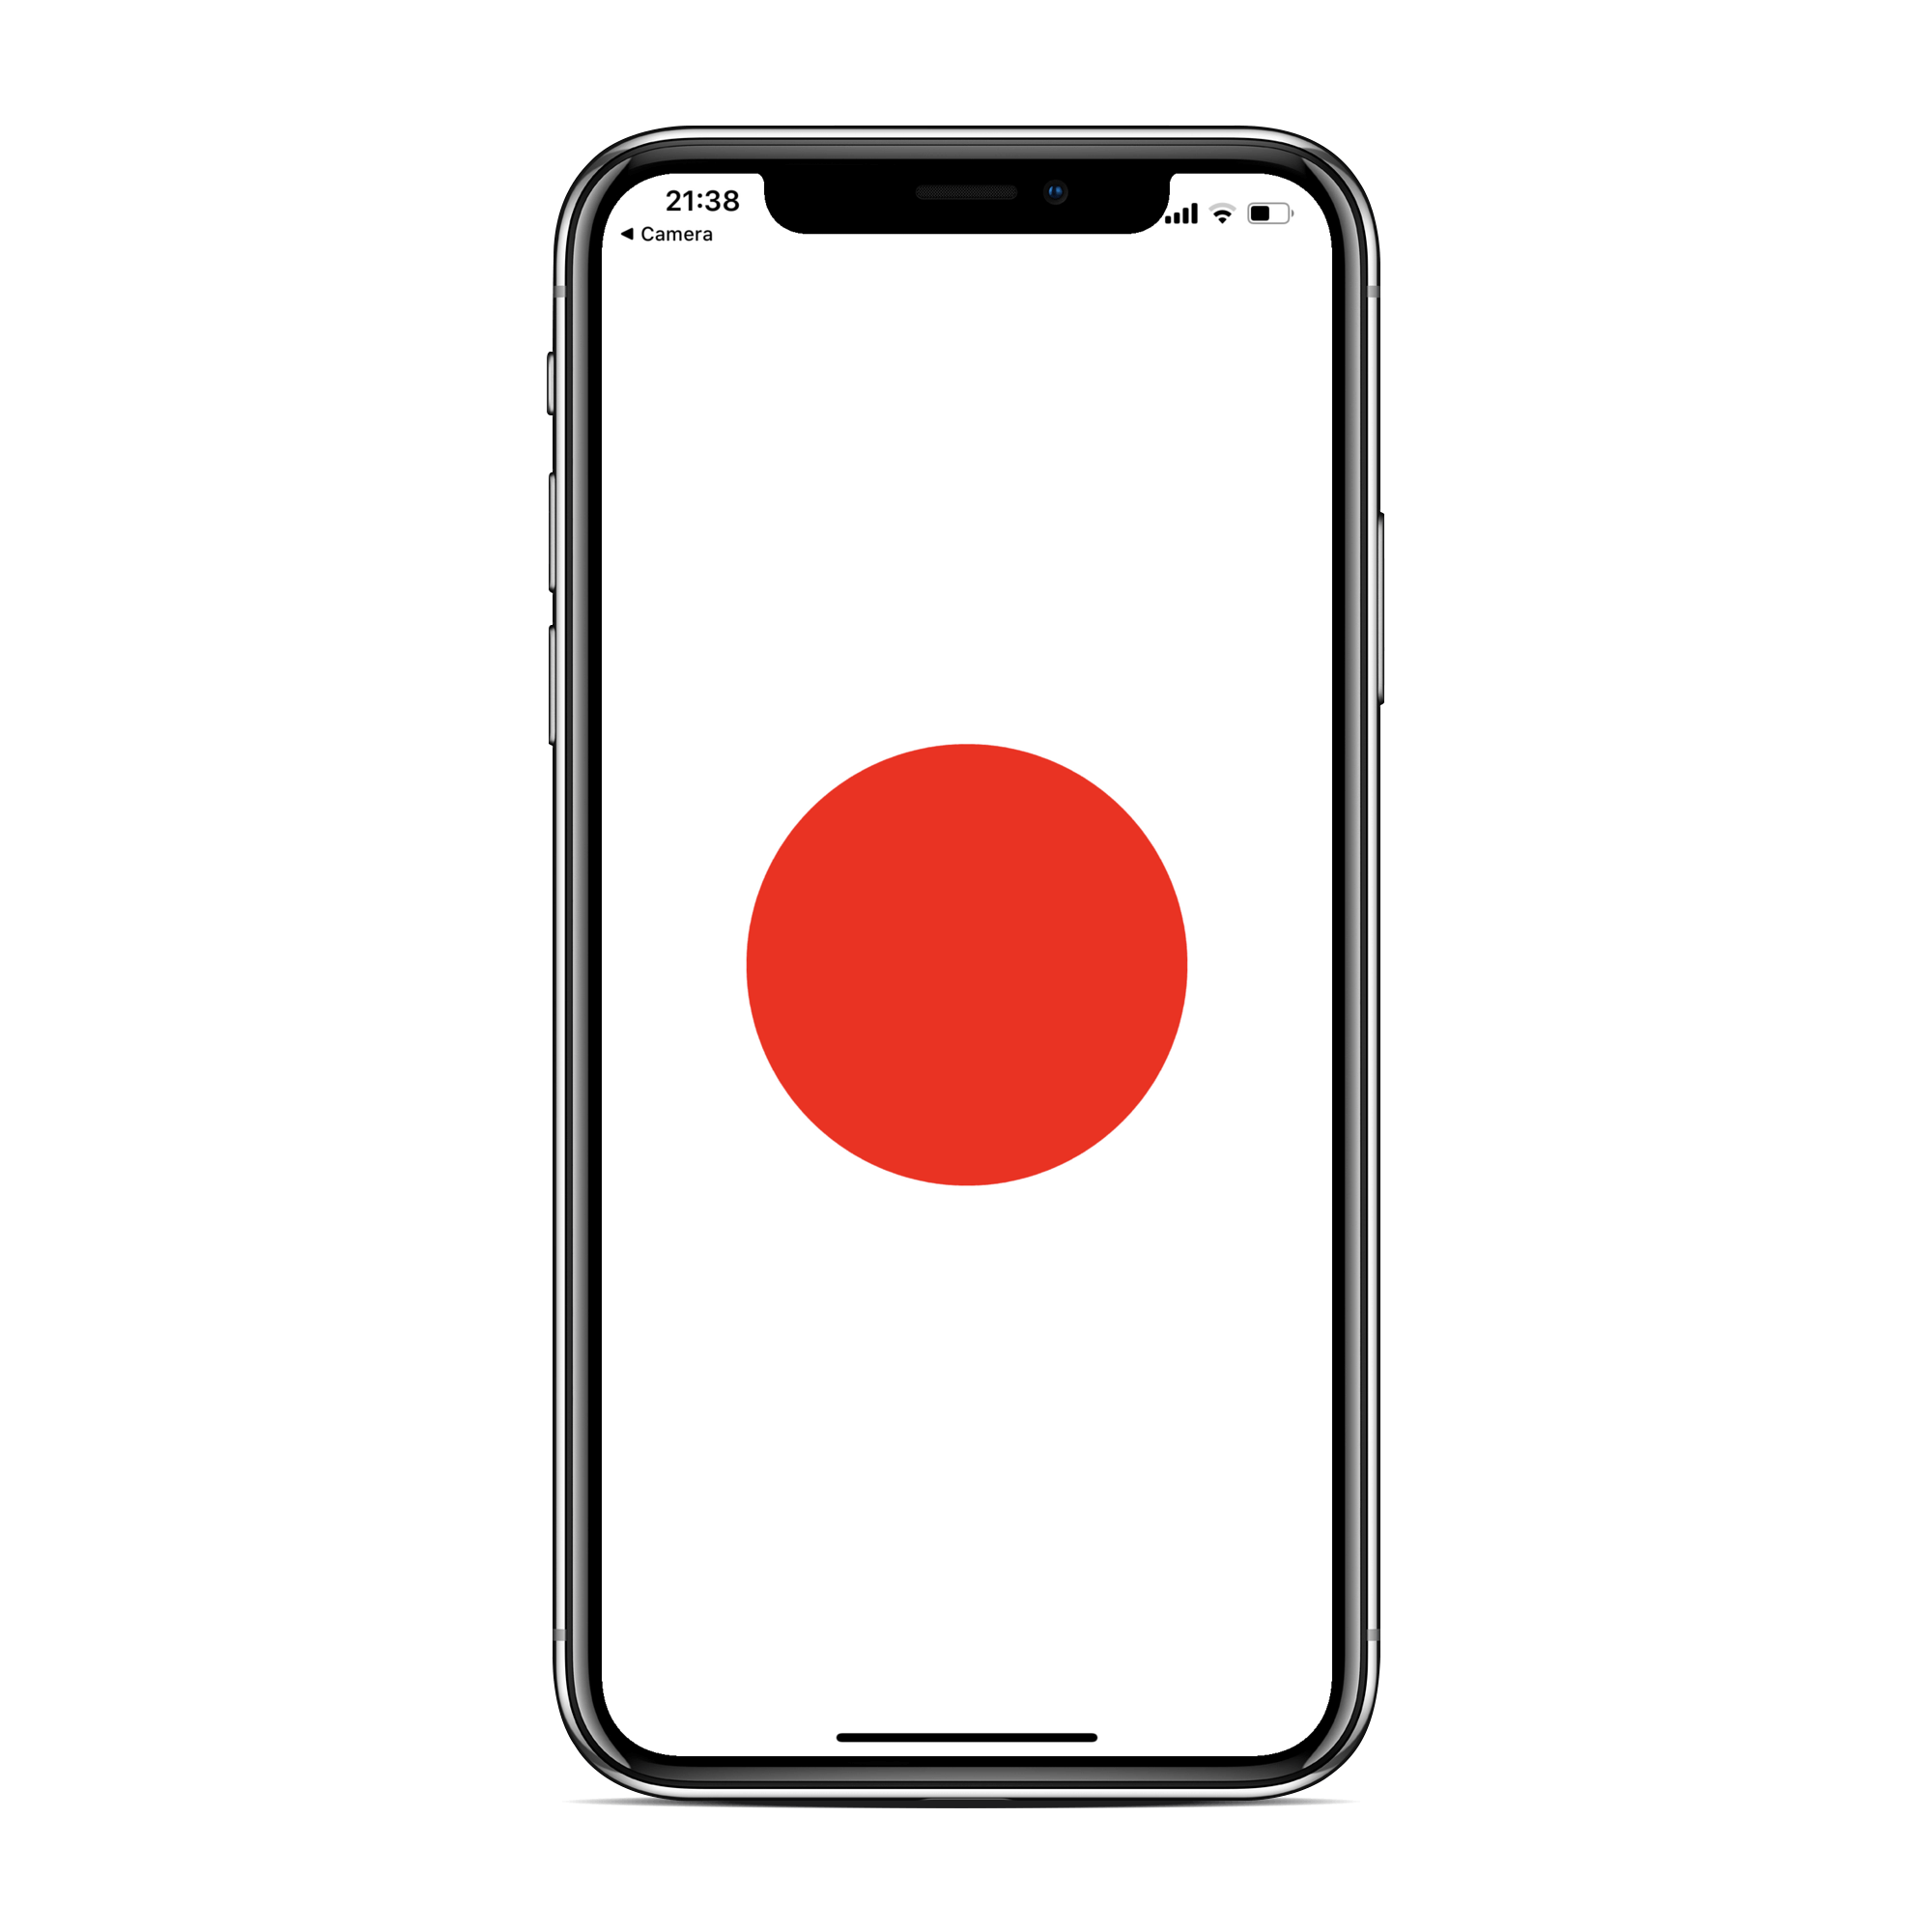
\includegraphics[width=0.25\textwidth]{max_kt1_images/image2.png} & 
            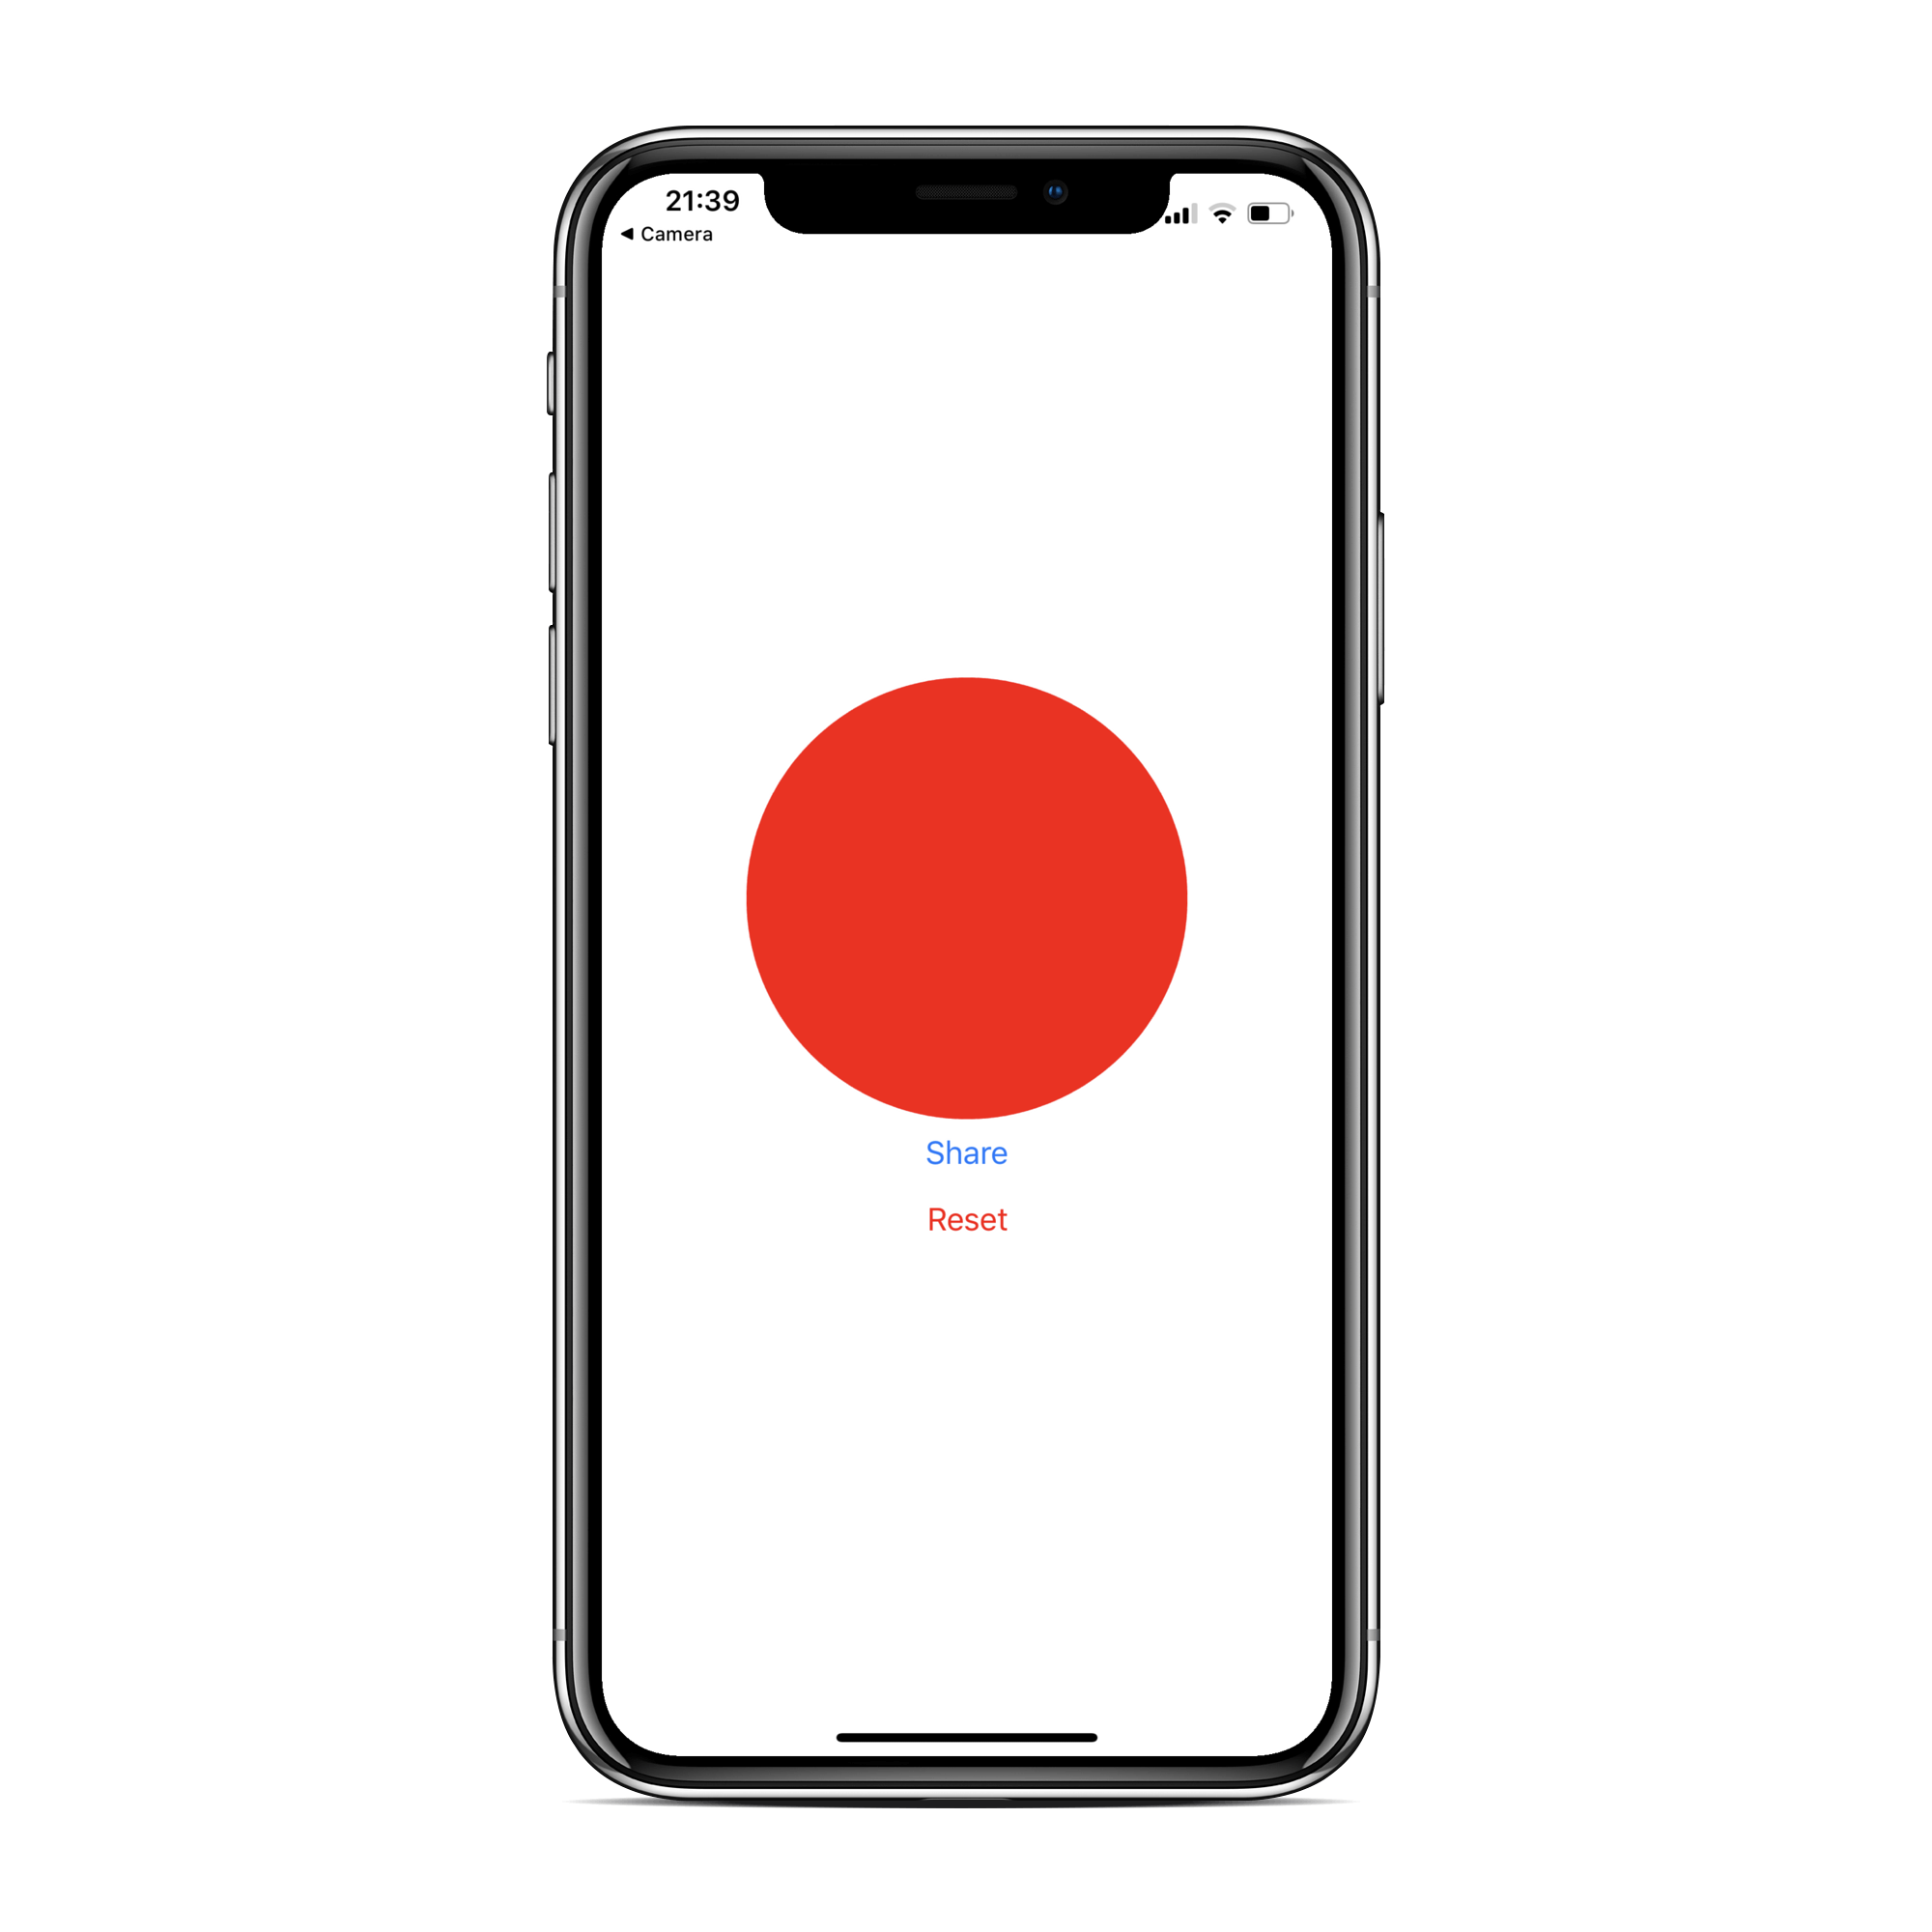
\includegraphics[width=0.25\textwidth]{max_kt1_images/image3.png} & 
            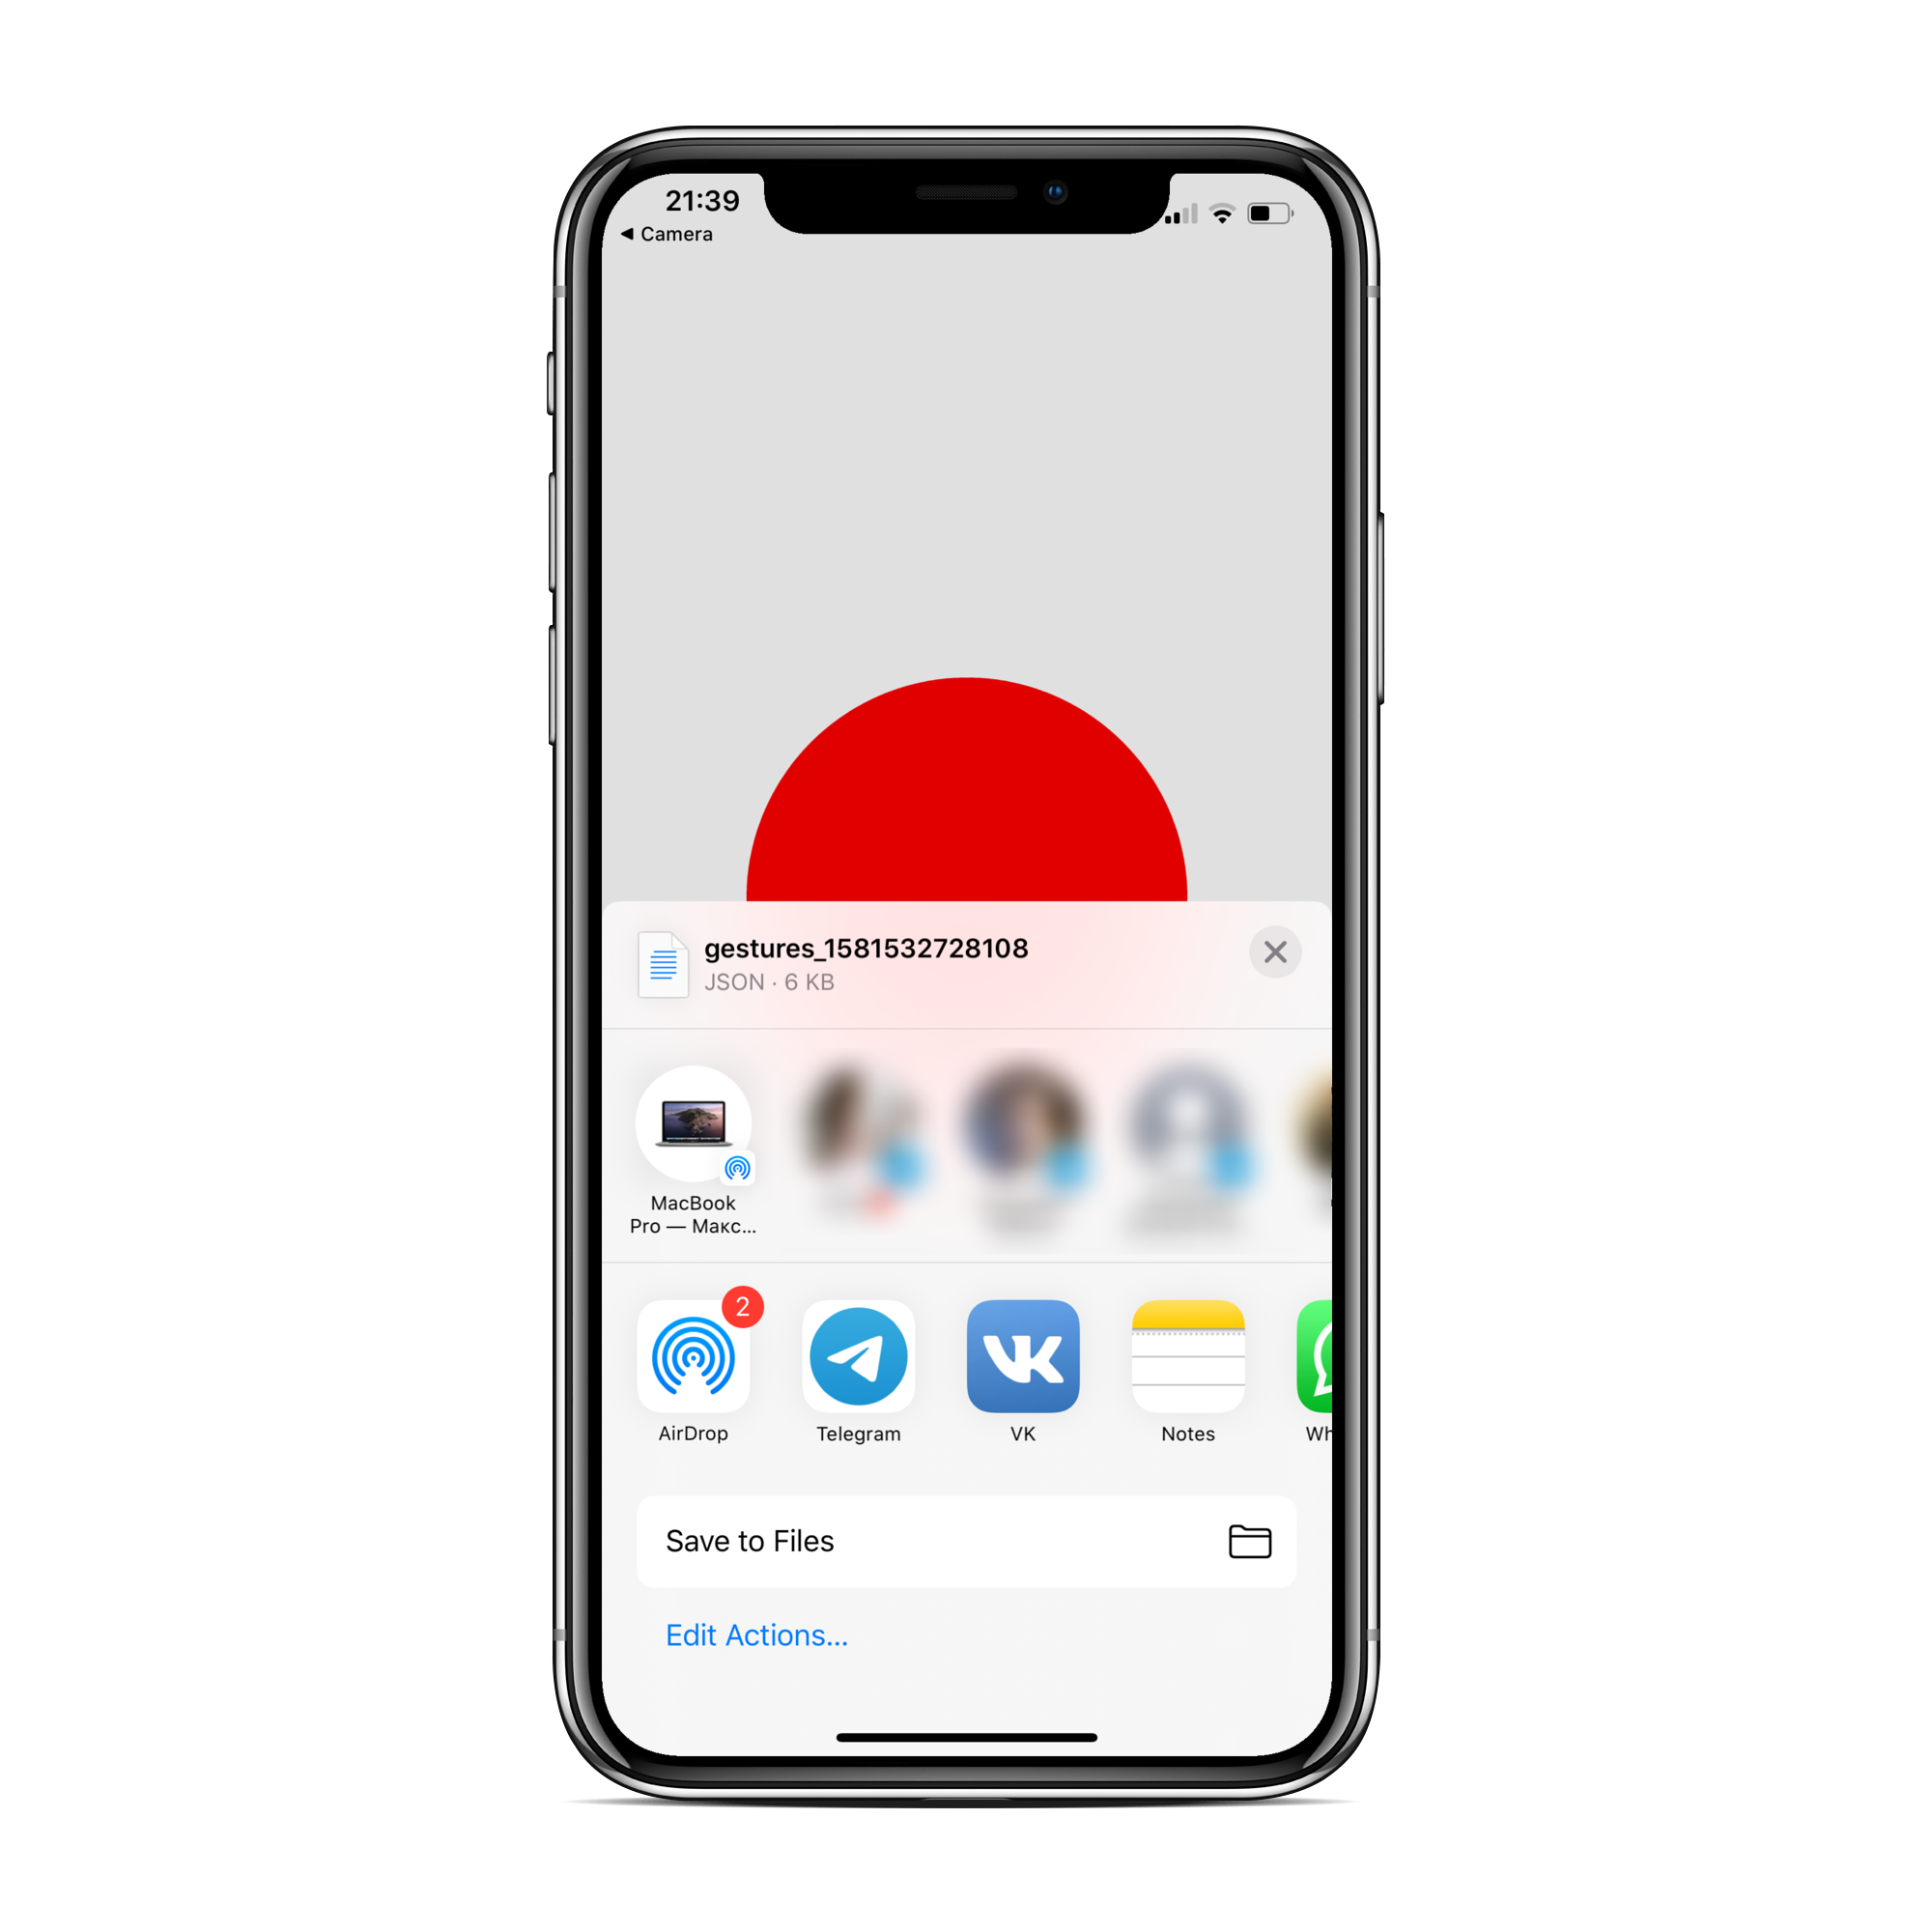
\includegraphics[width=0.25\textwidth]{max_kt1_images/image1.png} \\
        \end{tabular}
    \end{center}
    \caption{Интерфейс первой версии приложения.}
\end{figure}

% \subsection{КТ 2}

\subsection{Доработка приложения и первый прототип классификатора}
Далее, было необходимо доработать мобильное приложение. Также, несмотря на то что это не входило в список моих задач, я решил попробовать создать первый прототип классификатора обработанных данных.
% Моими основными задачами были доработка мобильного приложения и создание классификатора обработанных данных.
Так как обработанные данные есть ни что иное, как фигура на плоскости, было рассмотрено несколько вариантов классификации этих самых данных:
\begin{enumerate}
    \item Классифицировать фигуры без какой-либо дополнительной обработки
    \item Нормировать фигуры по максимальному отклонению от точки (0; 0)
    \item Построить графики с помощью программной библиотеки mathplotlib, после чего классифицировать полученные изображения
\end{enumerate}
В связи с тем, что классификация изображений является весьма распространенной задачей, то было решено выбрать следующую стратегию: строить графики показаний акселерометра с помощью программной библиотеки mathplotlib и классифицировать полученные изображения.

Таким образом, возникли следующие подзадачи:
\begin{enumerate}
    \item Построить графики с помощью программной библиотеки mathplotlib
    \item Классифицировать полученные изображения, используя методы машинного обучения
    \item Добавить вывод предсказаний в мобильное приложение
\end{enumerate}
Благодаря лабораторным работам по линейной алгебре имелся достаточно богатый опыт использования программной библиотеки mathplotlib, поэтому построение графиков не составило труда. Однако, необходимо было избавиться от посторонних данных на графиках, таких как шкалы и вспомогательные сетки, а также привести все данные к единому формату: квадратные изображения строго определенного размера, одинаковый масштаб по оси абсцисс и по оси ординат.

\begin{figure}[H]
    \begin{center}
        \begin{tabular}{cc}
            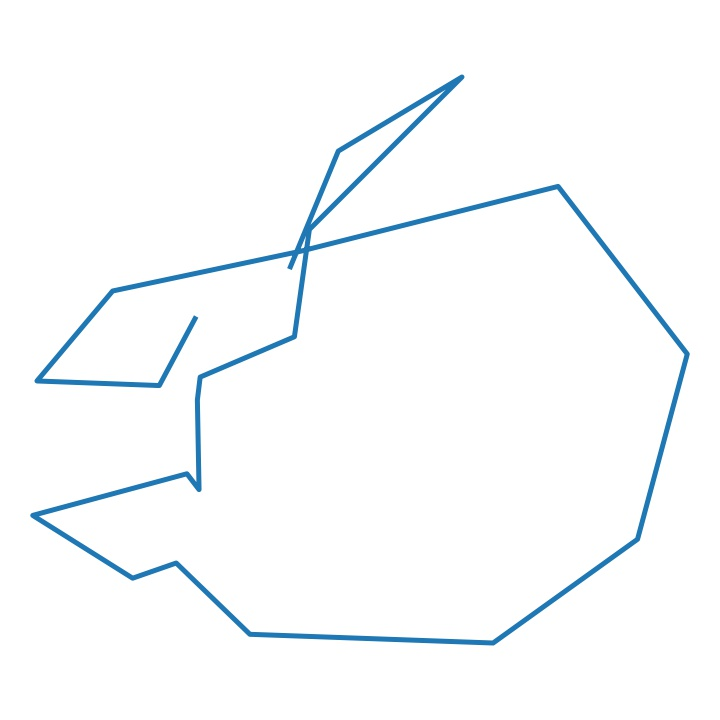
\includegraphics[width=0.4\textwidth]{max_kt2_images/image4.jpg} & 
            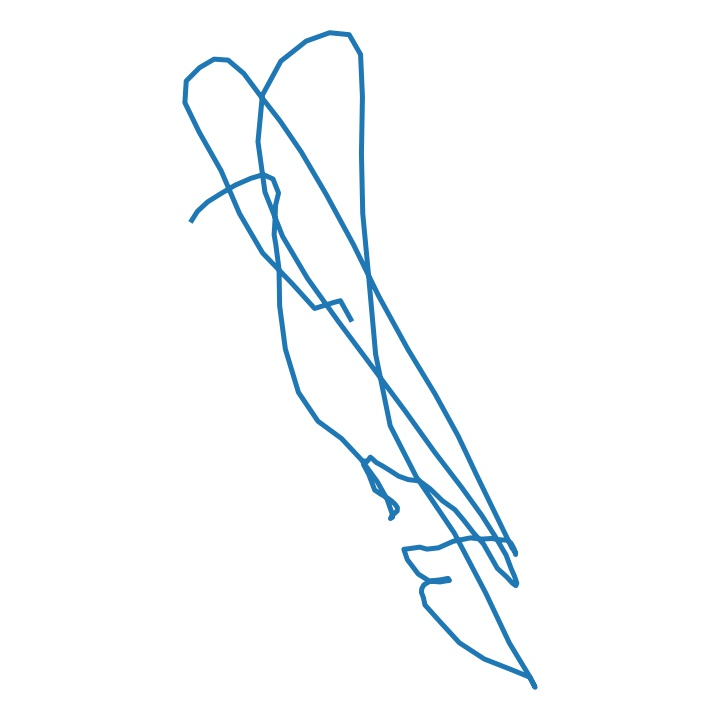
\includegraphics[width=0.4\textwidth]{max_kt2_images/image2.jpg} \\
        \end{tabular}
    \end{center}
    \caption{Примеры полученных изображений различных жестов: круг (слева), встряхивание (справа).}
\end{figure}

% Дополнительно, бонусом такого решения является то, что изображения нормируются по размеру автоматически.

Далее, я приступил к поиску подходящей программной библиотеки машинного обучения. Были рассмотрены следующие варианты:
\begin{enumerate}
    \item Theano -- библиотека численного вычисления в Python. Вычисления в Theano выражаются NumPy-подобным синтаксисом и компилируются для эффективных параллельных вычислений как на обычных CPU, так и на GPU.
    \item TensorFlow — открытая программная библиотека для машинного обучения, разработанная компанией Google для решения задач построения и тренировки нейронной сети с целью автоматического нахождения и классификации образов, достигая качества человеческого восприятия.
    \item Apache MXNet —  это программная платформа глубокого обучения с открытым исходным кодом, используемая для обучения и развертывания глубоких нейронных сетей.
\end{enumerate}

В связи с популярностью программной библиотеки TensorFlow и, как следствие, обилием готовых решений, основанных на ней, выбор был очевиден. Также данная библиотека является достаточно производительной, так как вся работа ведется с графами вычислений, операции с которыми, можно эффективно исполнять на некоторых типах процессоров.  Так как опыта работы с TensorFlow у меня не было совсем, первым делом было решено искать примеры проектов, сделанных на основе этой программной библиотеки. В процессе поиска я наткнулся на очень интересное решение от Google – Teachable Machine. Это инструмент, основанный на веб-технологиях, который делает обучение моделей быстрым, легким и доступным каждому, а также позволяет экспортировать полученные модели для интеграции в собственные решения.

\begin{figure}[H]
    \begin{center}
        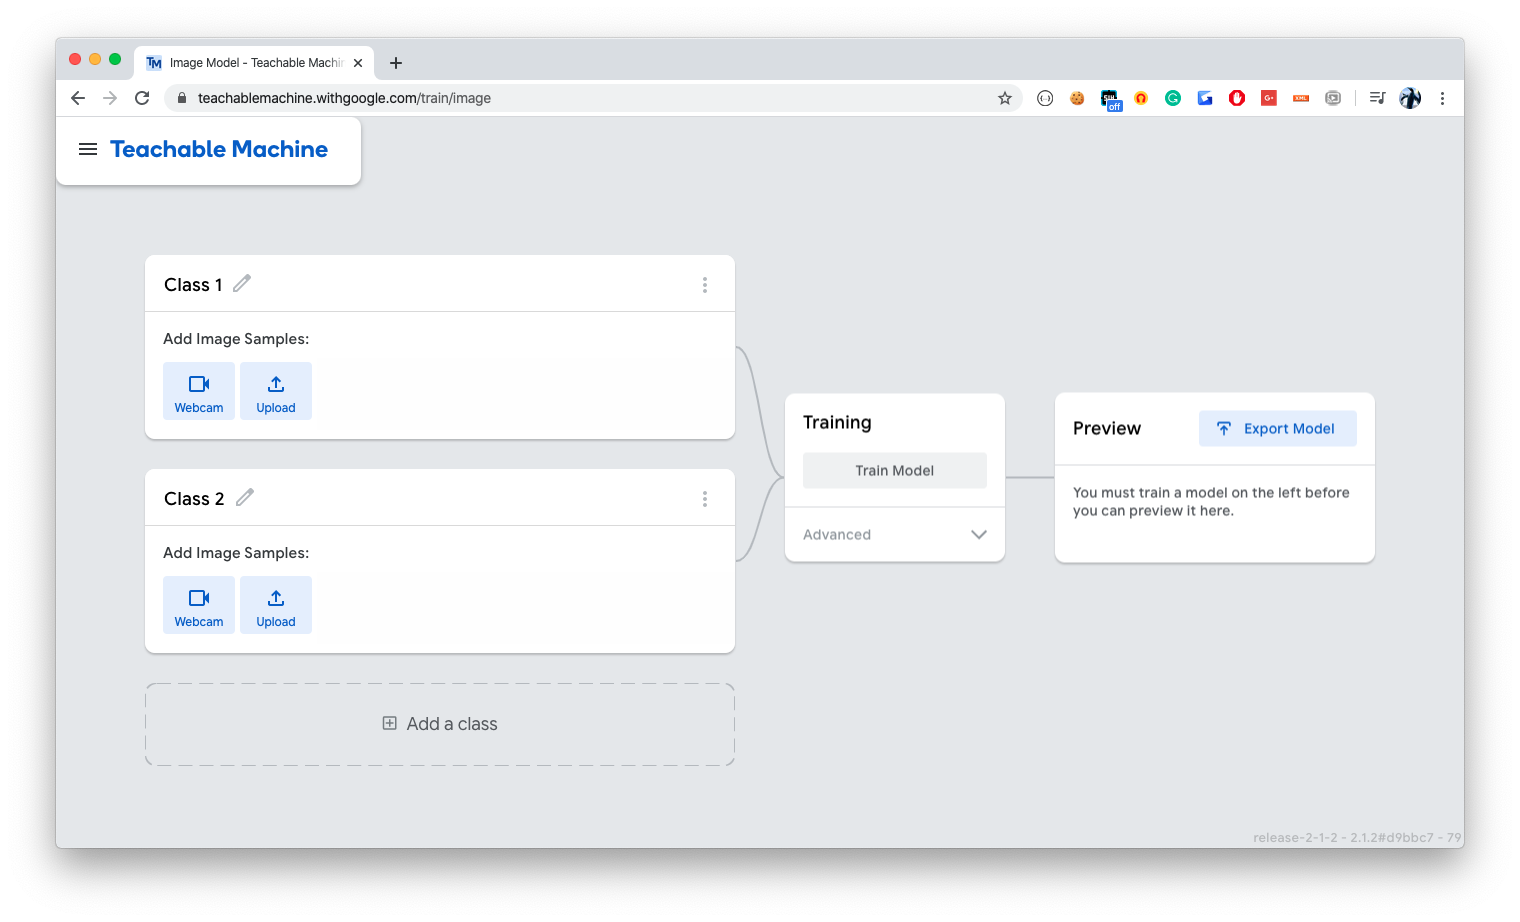
\includegraphics[width=0.8\textwidth]{max_kt2_images/image10.png}
    \end{center}
    \caption{Интерфейс программы “Teachable Machine”.}
\end{figure}

В программе предустановлены 3 модели: для распознавания изображений, аудиозаписей и поз. Нас интересует первая модель – это сверточная нейронная сеть. Данный тип искусственных нейронных нейронных сетей хорошо зарекомендовал себя в задачах распознавания образов. Главное отличие сверточных нейронных сетей от обыкноневенного перцептрона, то есть полносвязной нейронной сети, в том, что она обучается на основе карт признаков, которые формируются в результате операций свертки матрицами весов различных фильтров. Сами же матрицы весов корректируются в процессе обучения методом обратного распространения ошибки.

\begin{figure}[H]
    \begin{center}
        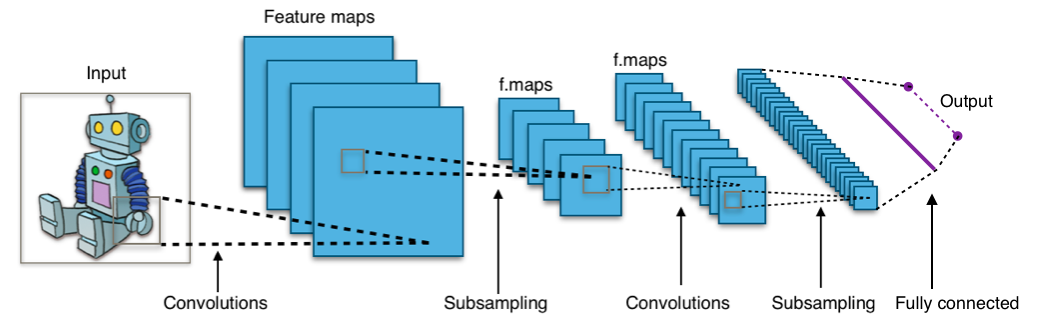
\includegraphics[width=0.8\textwidth]{max_kt2_images/image7.png}
    \end{center}
    \caption{Типовая архитектура сверточной нейронной сети.}
\end{figure}

% Принцип работы Teachable Machine прост: в левом меню создаются классы и для каждого загружается набор тренировочных изображений или аудиозаписей в зависимости от выбранного ранее типа модели. При необходимости можно указать дополнительные параметры обучения (скорость обучения, количество эпох и т.д.), однако, как выяснилось позже, стандартные параметры обучения позволяют добиться достаточно неплохих результатов. Затем, полученную модель можно экспортировать в формате “.h5”.

Далее, нужно было определиться с классами движений. После совещания с другими участниками команды, мы остановились на том, что система будет уметь распознавать три типа жестов: круг, квадрат и встряхивание. Недолго думая, один из участников команды приступил к сбору датасета и уже через пару часов, в моих руках было 15 экземпляров “кругов”, 14 “квадратов” и столько же “встряхиваний”. Далее, данный набор данных был загружен в Teachable Machine, а также была запущена тренировка со стандартными настройками (50 эпох, batch size = 16, скорость обучения = 0,001).  После чего, модель была экспортирована для использования вместе с интерпретируемым языком программирования Python 3. Сразу же захотелось протестировать данную модель: из другого набора данных были выбраны несколько записанных ранее жестов в виде графиков, которые после стали входными данными для алгоритма распознавания. Были получены следующие результаты:

\begin{figure}[H]
    \begin{center}
        \begin{tabular}{cc}
            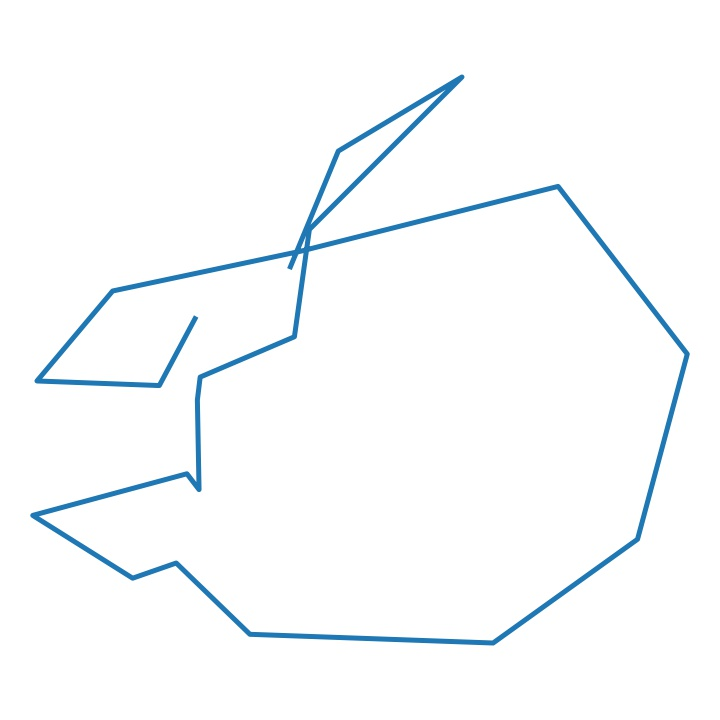
\includegraphics[width=0.35\textwidth]{max_kt2_images/image4.jpg} & 
            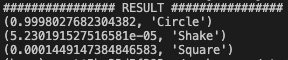
\includegraphics[width=0.35\textwidth]{max_kt2_images/image11.png} \\
        \end{tabular}
    \end{center}
    \caption{Исходное изображение круга (слева) и результат работы алгоритма (справа).}
\end{figure}

\begin{figure}[H]
    \begin{center}
        \begin{tabular}{cc}
            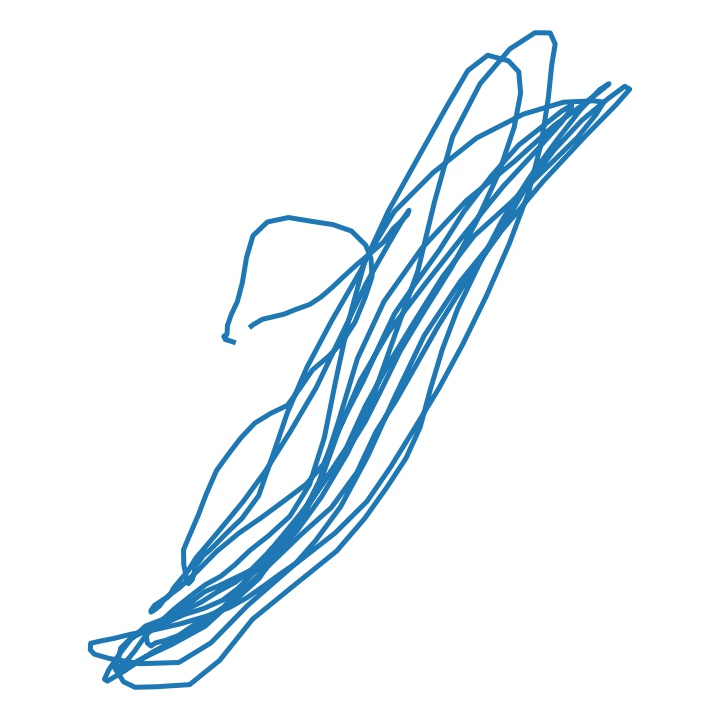
\includegraphics[width=0.35\textwidth]{max_kt2_images/image9.jpg} & 
            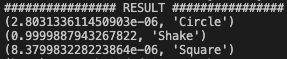
\includegraphics[width=0.35\textwidth]{max_kt2_images/image8.png} \\
        \end{tabular}
    \end{center}
    \caption{Исходное изображение встряхивания (слева) и результат работы алгоритма (справа).}
\end{figure}

\begin{figure}[H]
    \begin{center}
        \begin{tabular}{cc}
            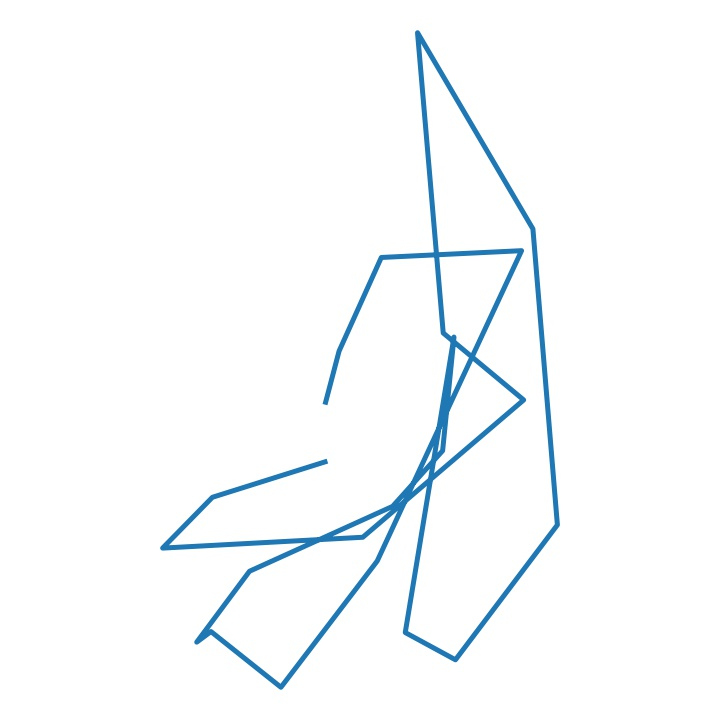
\includegraphics[width=0.35\textwidth]{max_kt2_images/image3.jpg} & 
            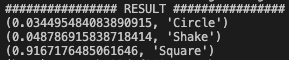
\includegraphics[width=0.35\textwidth]{max_kt2_images/image1.png} \\
        \end{tabular}
    \end{center}
    \caption{Исходное изображение квадрата (слева) и результат работы алгоритма (справа).}
\end{figure}

Также, хотелось бы видеть результат распознавания сразу после записи какого-либо жеста, для чего было решено сделать http сервер на node.js и доработать мобильное приложение так, чтобы оно отправляло записанное движение на данный сервер, а сервер в свою очередь запускал алгоритм распознавания и возвращал результат его работы обратно в приложение.

% В процессе реализации вышеперечисленного возникла следующая проблема: распознавание происходило слишком медленно, так как при каждом запросе на сервер происходила загрузка модели в оперативную память. Решение лежит на поверхности: для корректной работы необходимо загрузить модель в оперативную память всего 1 раз, а значит нужно сделать так, чтобы алгоритм распознавания не завершался после каждого распознавания, а ждал следующего запроса. Однако, текущее решение не позволяло достаточно быстро совершить модернизацию такого рода, из-за чего пришлось использовать протокол удаленного вызова процедур XML-RPC для связи между веб-сервером и алгоритмом распознавания (ранее данные передавались через стандартные потоки ввода/вывода). Усовершенствованная система работала значительно быстрее.

\begin{figure}[H]
    \begin{center}
        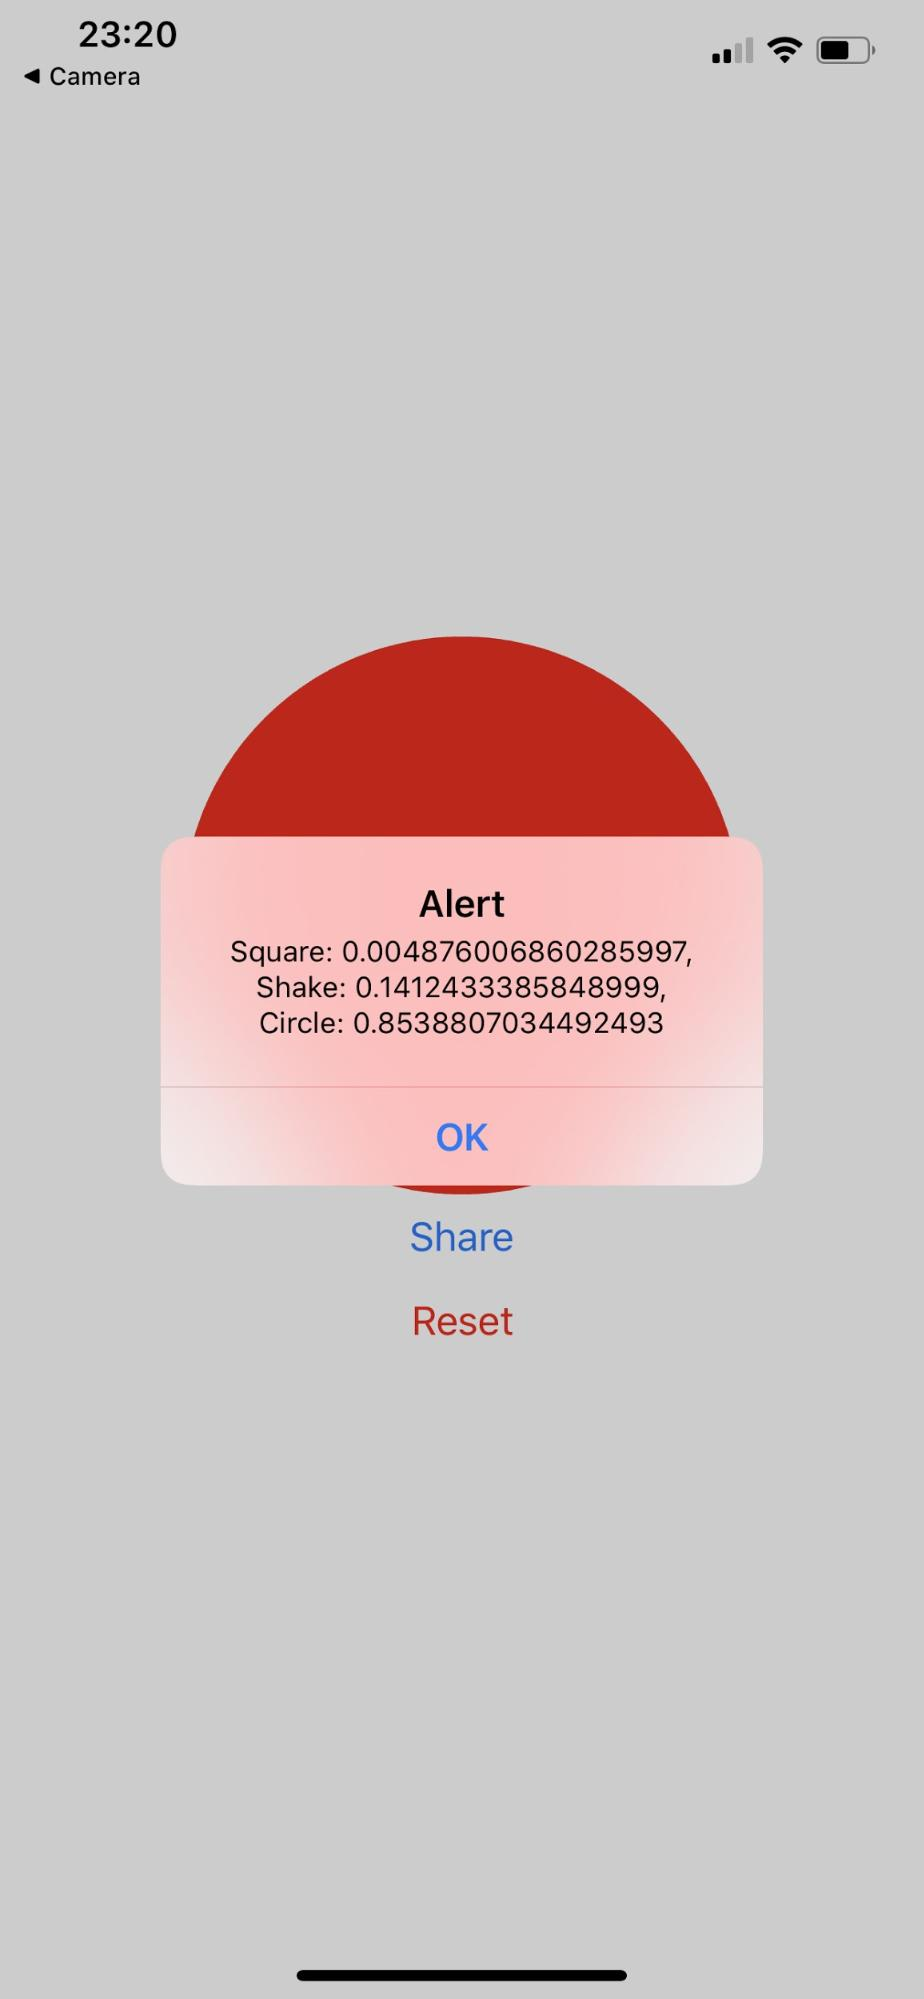
\includegraphics[width=0.3\textwidth]{max_kt2_images/image5.jpg}
    \end{center}
    \caption{Интерфейс усовершенствованного мобильного приложения. Снимок экрана был сделан сразу после записи движения.}
\end{figure}

\subsection{Последняя версия}
Затем, в связи с наличием практически полностью готовой библиотеки для обучения и распознавания жестов, разработанной одним из участников нашей команды, было решено все-таки переделать приложение, чтобы повысить удобство его использования. Пришлось практически полностью переработать интерфейс. Теперь приложение имеет две вкладки: тренировка и распознавание. Они отвечают, как следует из названия, за тренировку и распознавание соответственно.

Тестирование происходит следующим образом: зажимается кнопка \textit{Record} и выполняется движение. Далее приложение, используя программную библиотеку, получает результат распознавания. В результате чего на экране появляется изображение восстановленного жеста и предсказание алгоритма в виде надписи вида \textit{"I guess it's a <название жеста>"}. Далее, при желании можно нажать на кнопку \textit{Reset}, чтобы записать новый жест.
\begin{figure}[H]
    \begin{center}
        \begin{tabular}{ccc}
            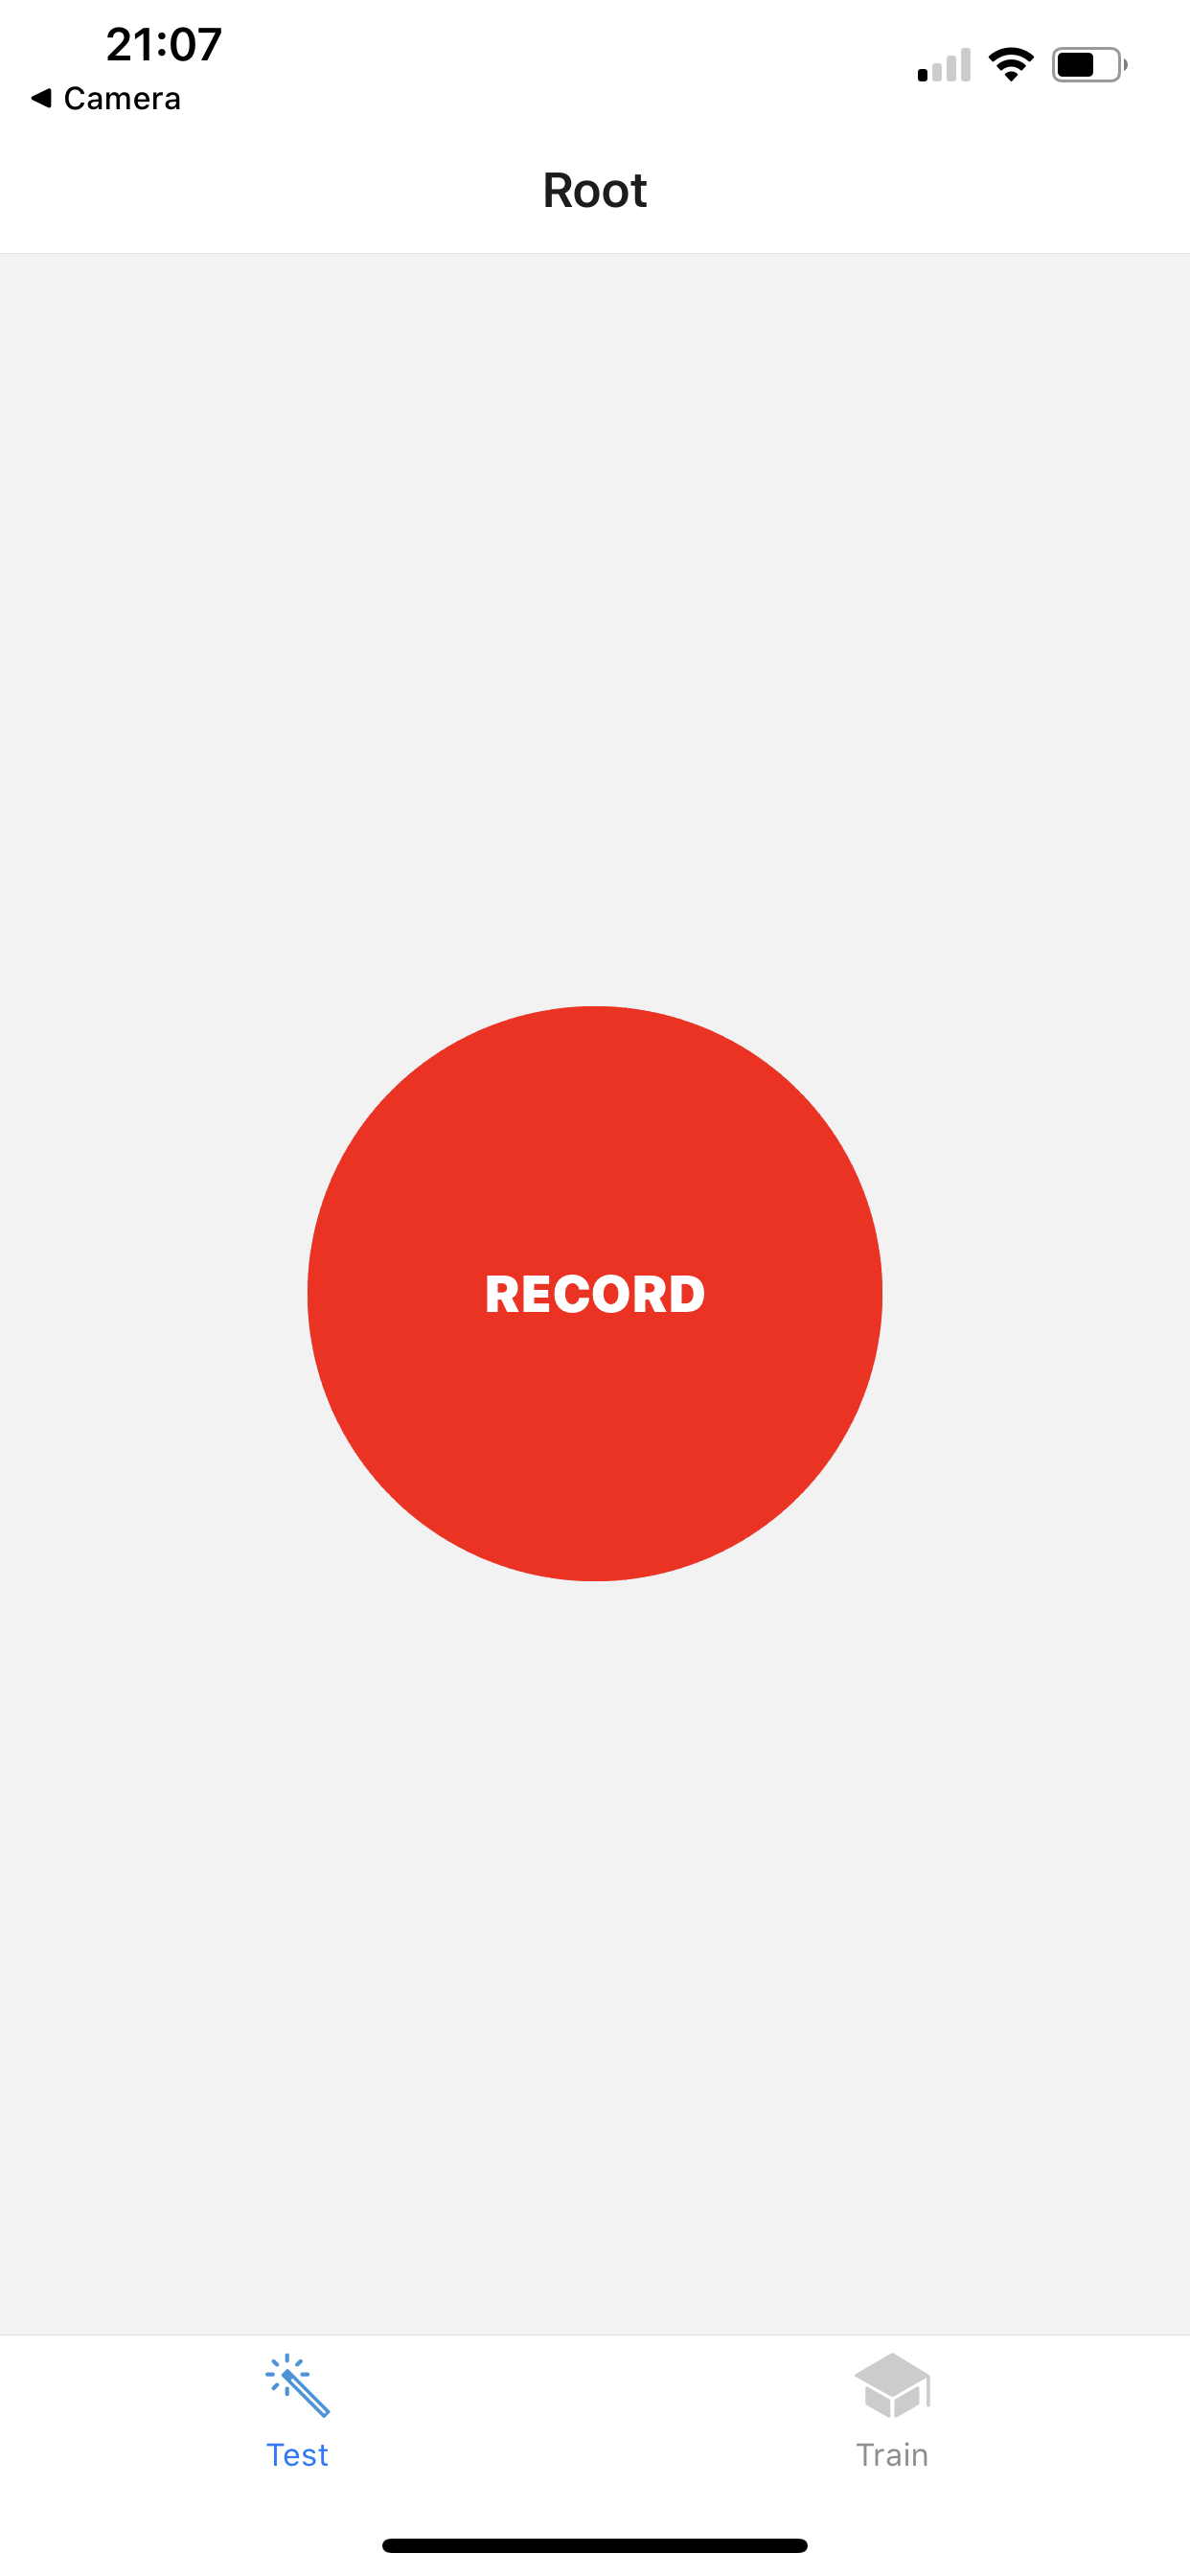
\includegraphics[width=0.15\textwidth]{testingapp_screenshots/IMG_2011.PNG} & 
            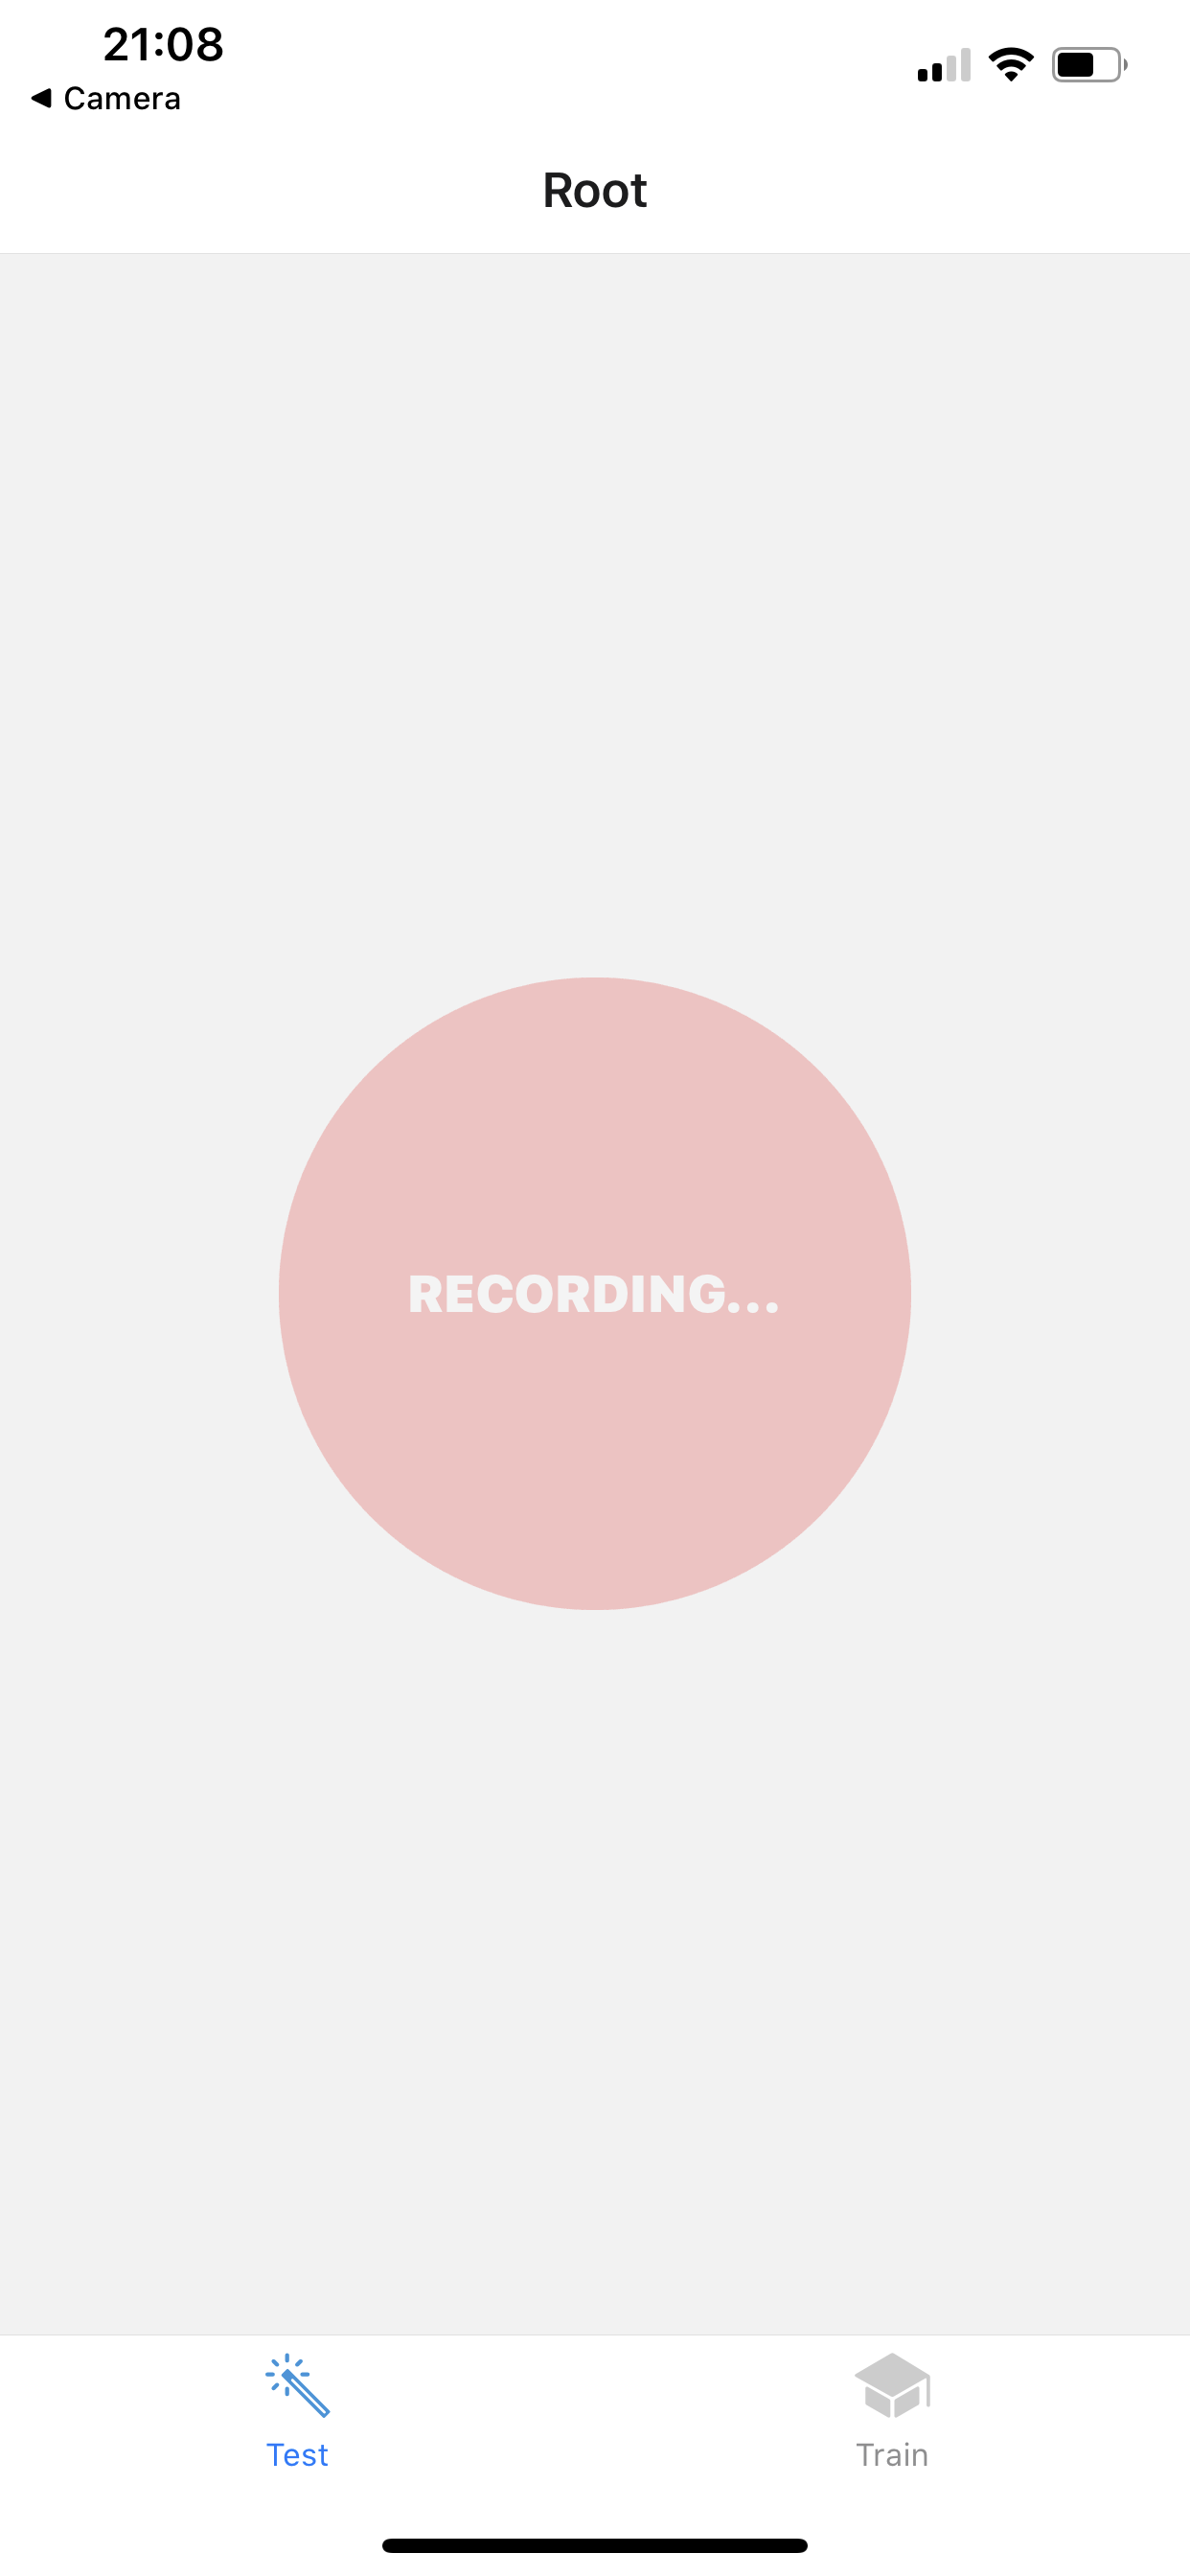
\includegraphics[width=0.15\textwidth]{testingapp_screenshots/IMG_2016.PNG} & 
            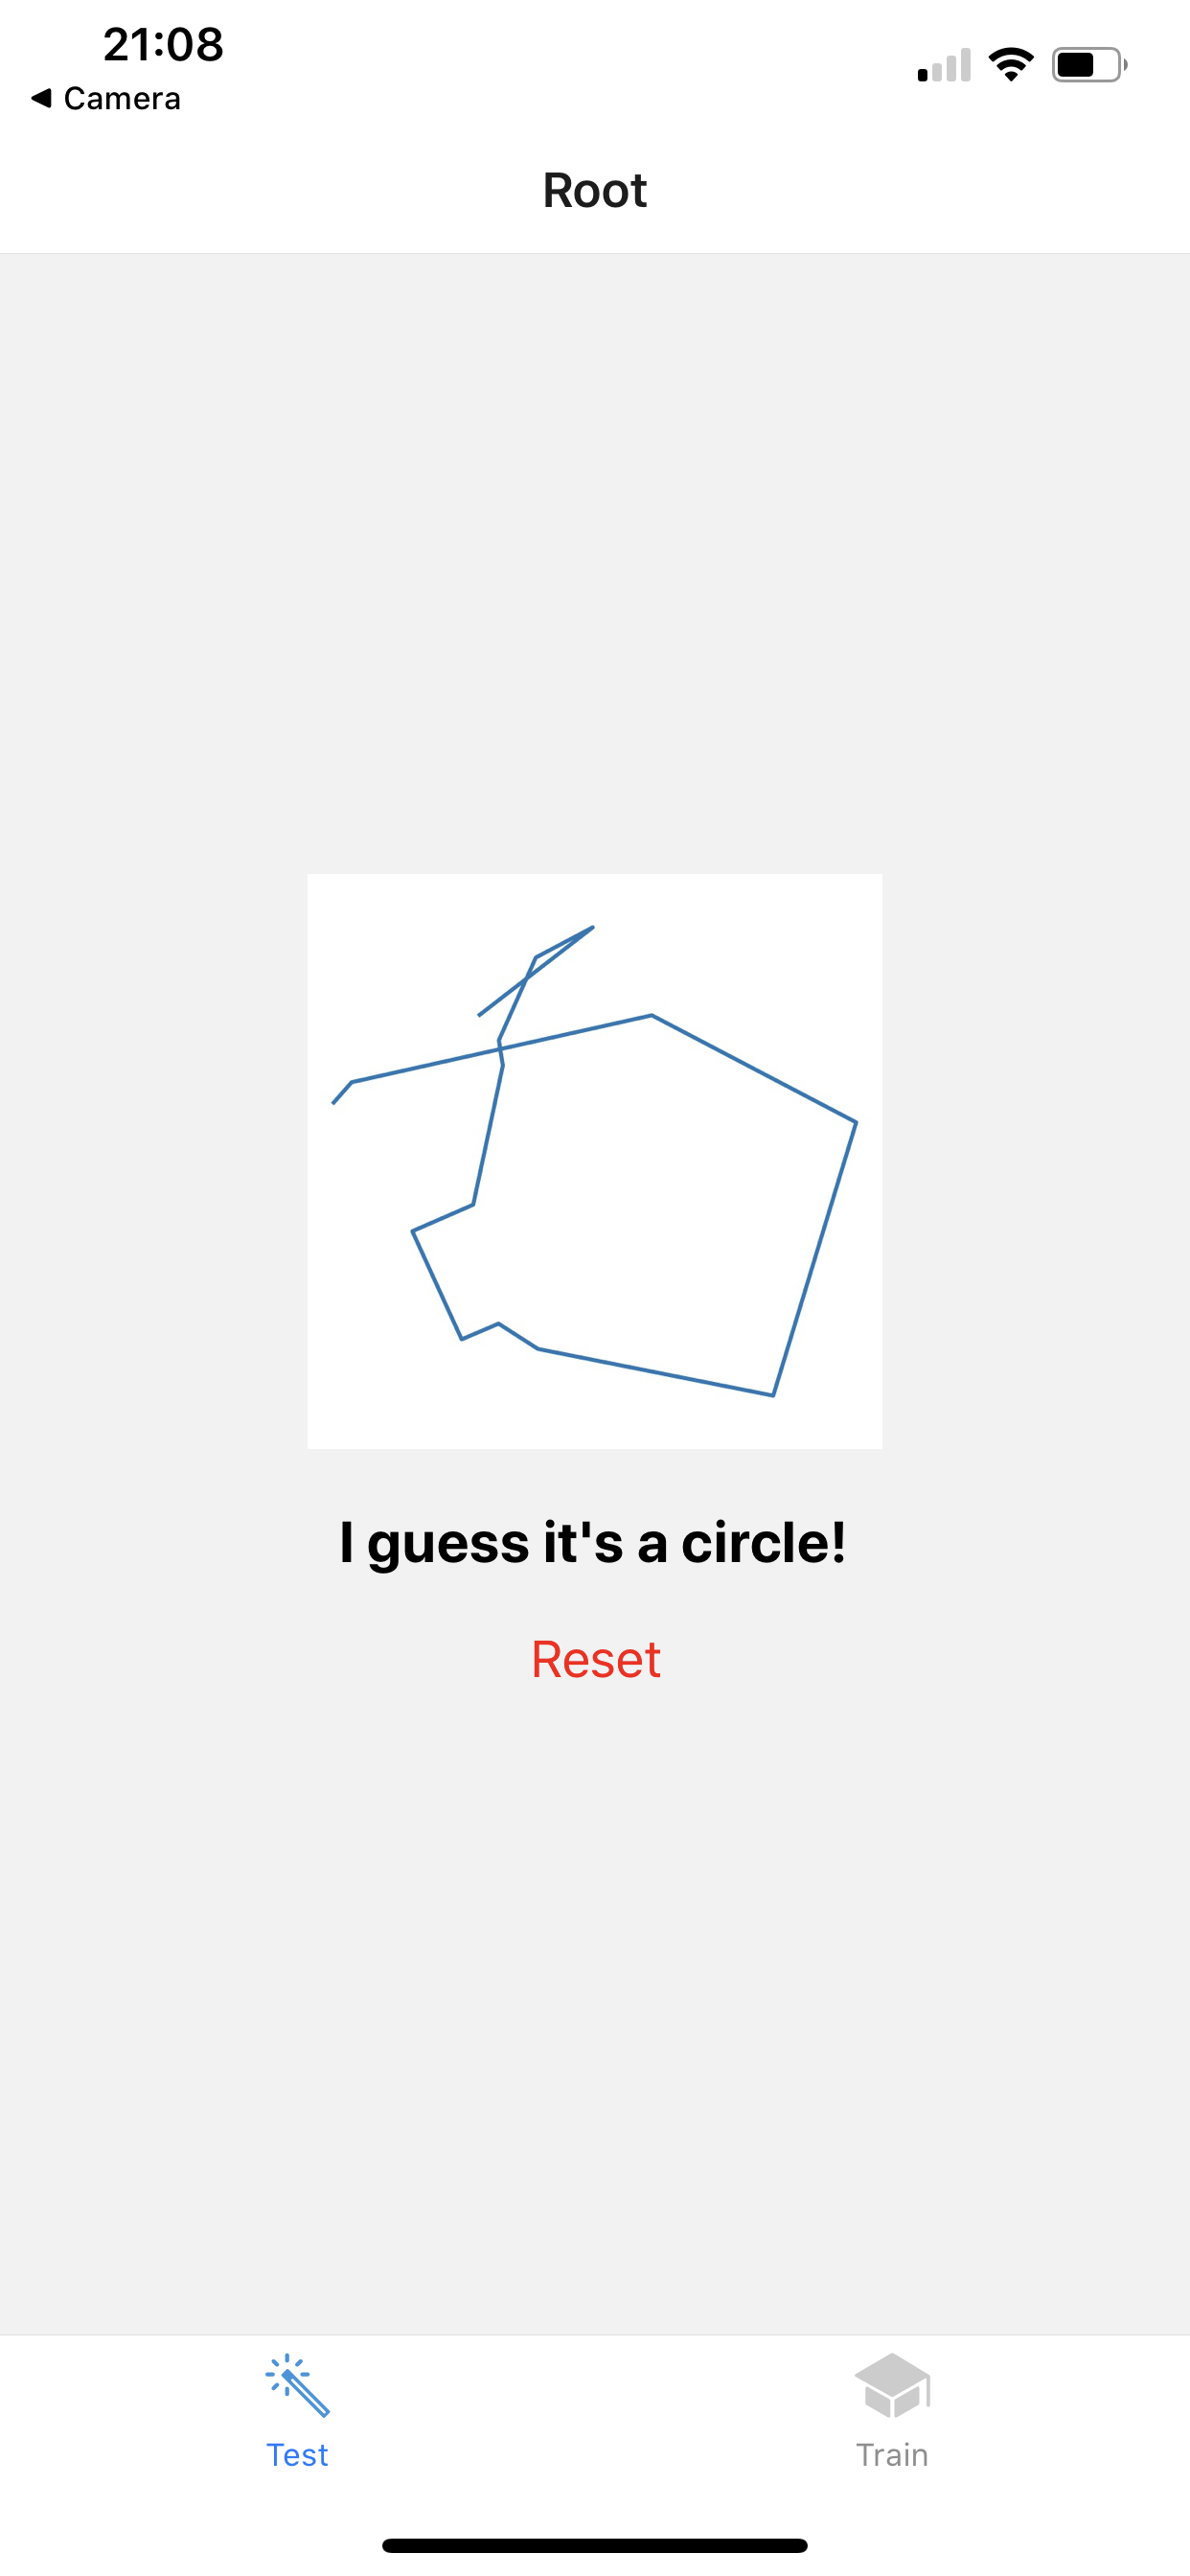
\includegraphics[width=0.15\textwidth]{testingapp_screenshots/IMG_2017.PNG} \\
        \end{tabular}
    \end{center}
    \caption{Интерфейс тестирования в различных состояниях.}
\end{figure}

Процесс обучения немного отличается: жест записывается аналогичным образом, но после записи жеста появляются 3 кнопки: \textit{Reset, Submit} и \textit{Share}. Первая кнопка работает тем же образом, что и при тестировании, третья отвечает за отправку записанного жеста с помощью AirDrop, Telegram, электронной почты и т.д. При нажатии на кнопку \textit{Submit} записанные данные с помощью программной библиотеки отправляются на сервер, а он в свою очередь возвращает изображение жеста восстановленное из этих данных. Затем, оно появляется на месте кнопки записи жеста.
\begin{figure}[H]
    \begin{center}
        \begin{tabular}{cccc}
            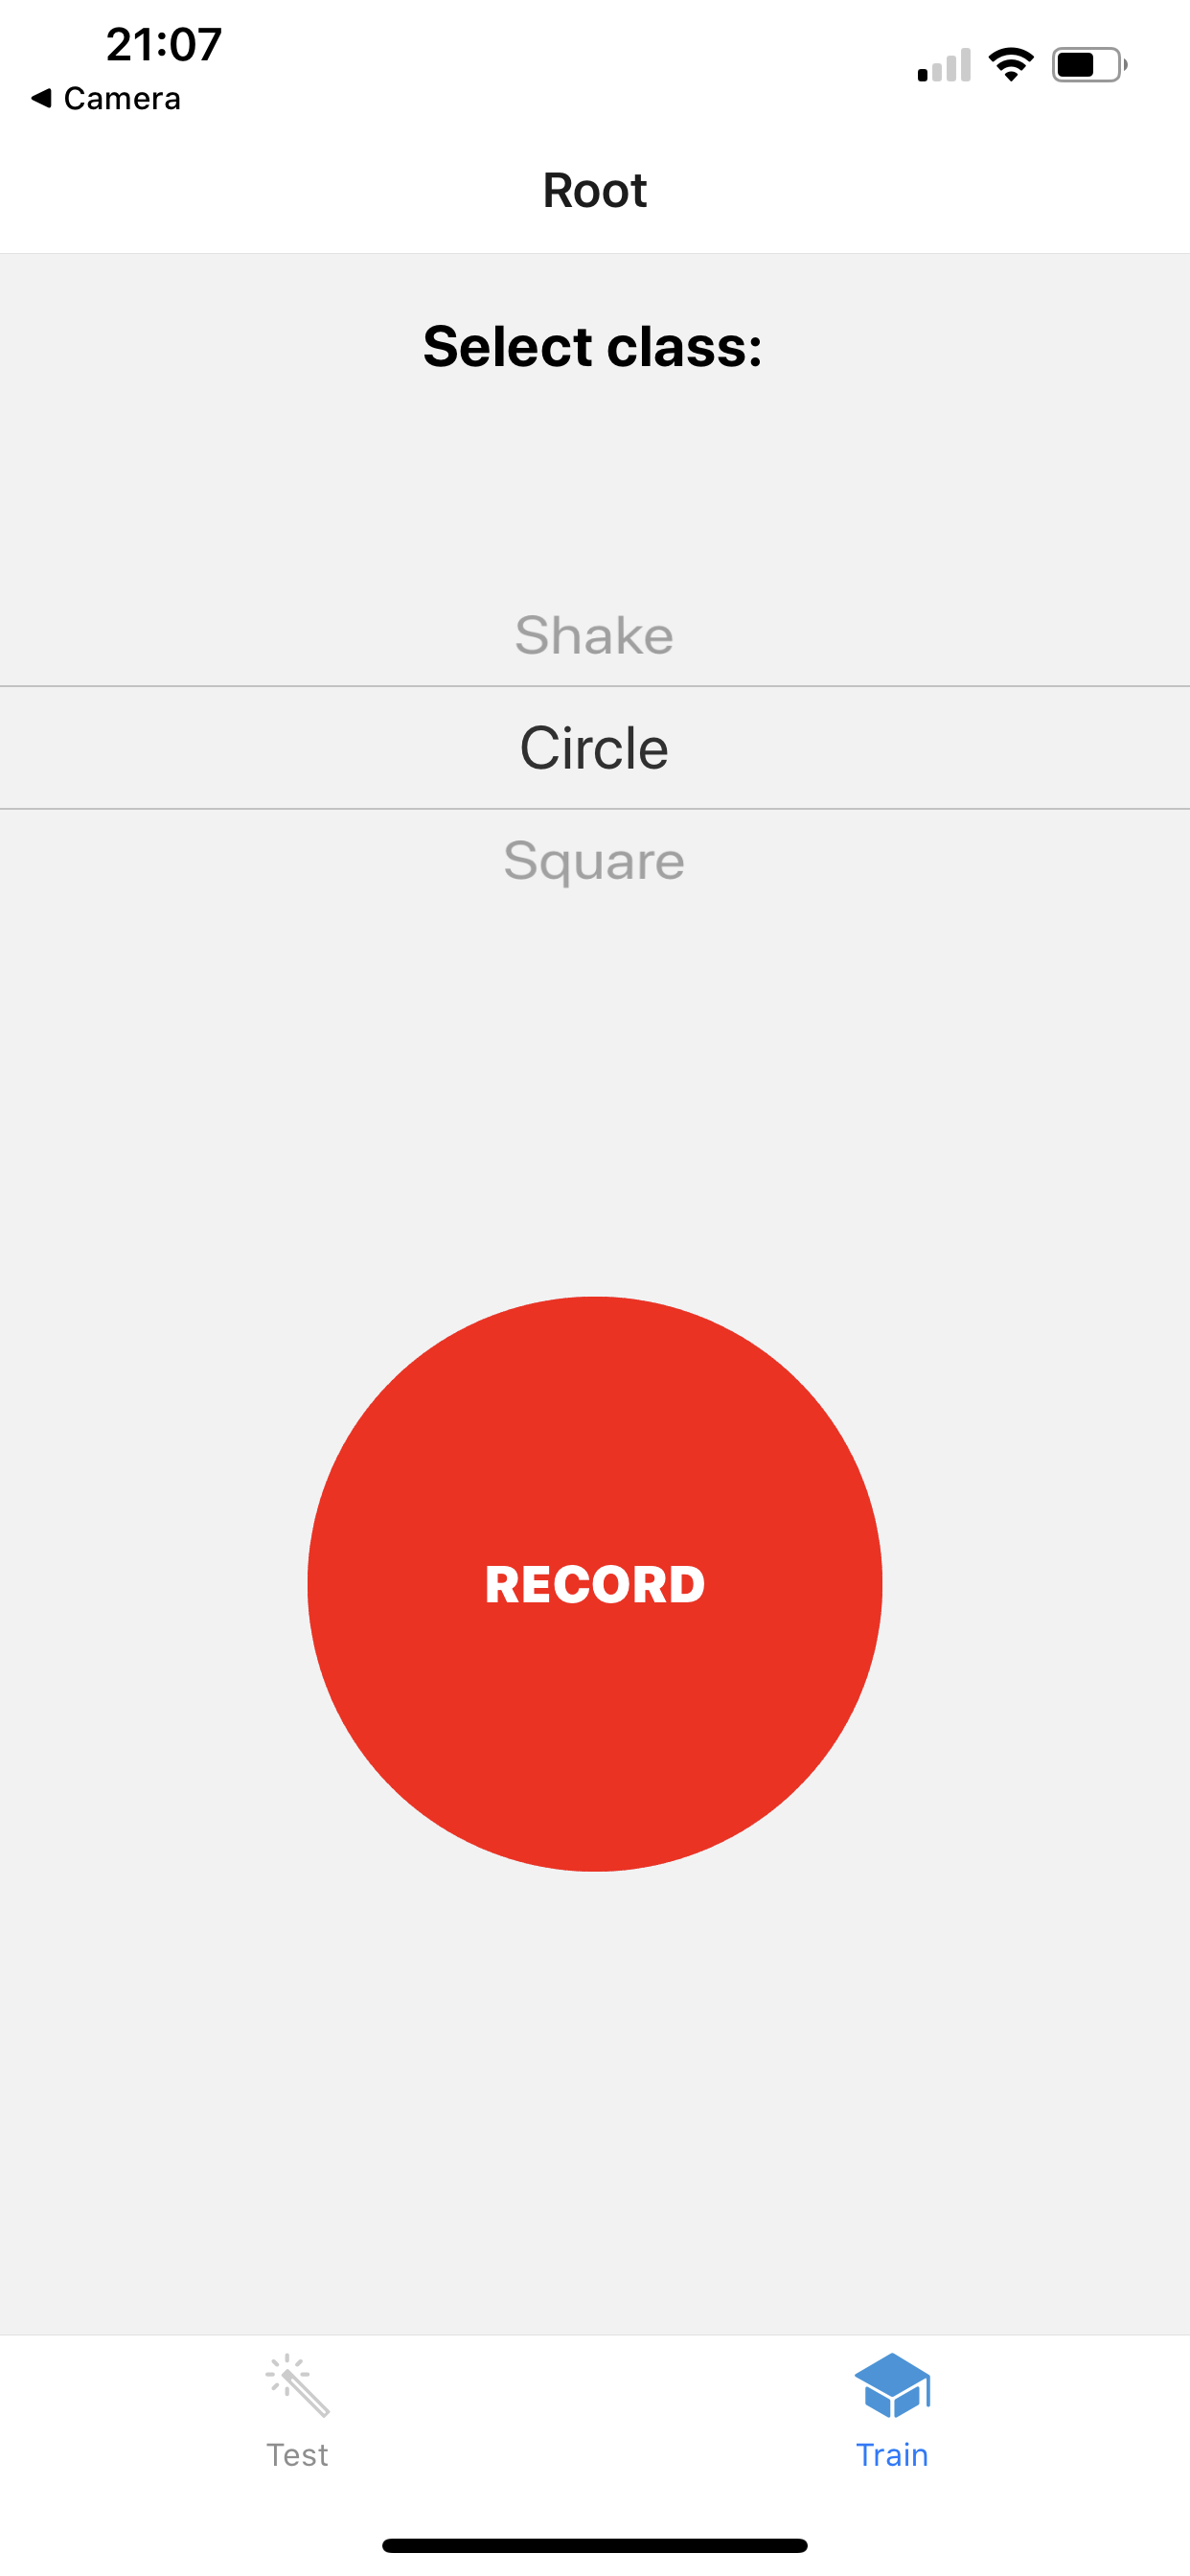
\includegraphics[width=0.15\textwidth]{testingapp_screenshots/IMG_2012.PNG} & 
            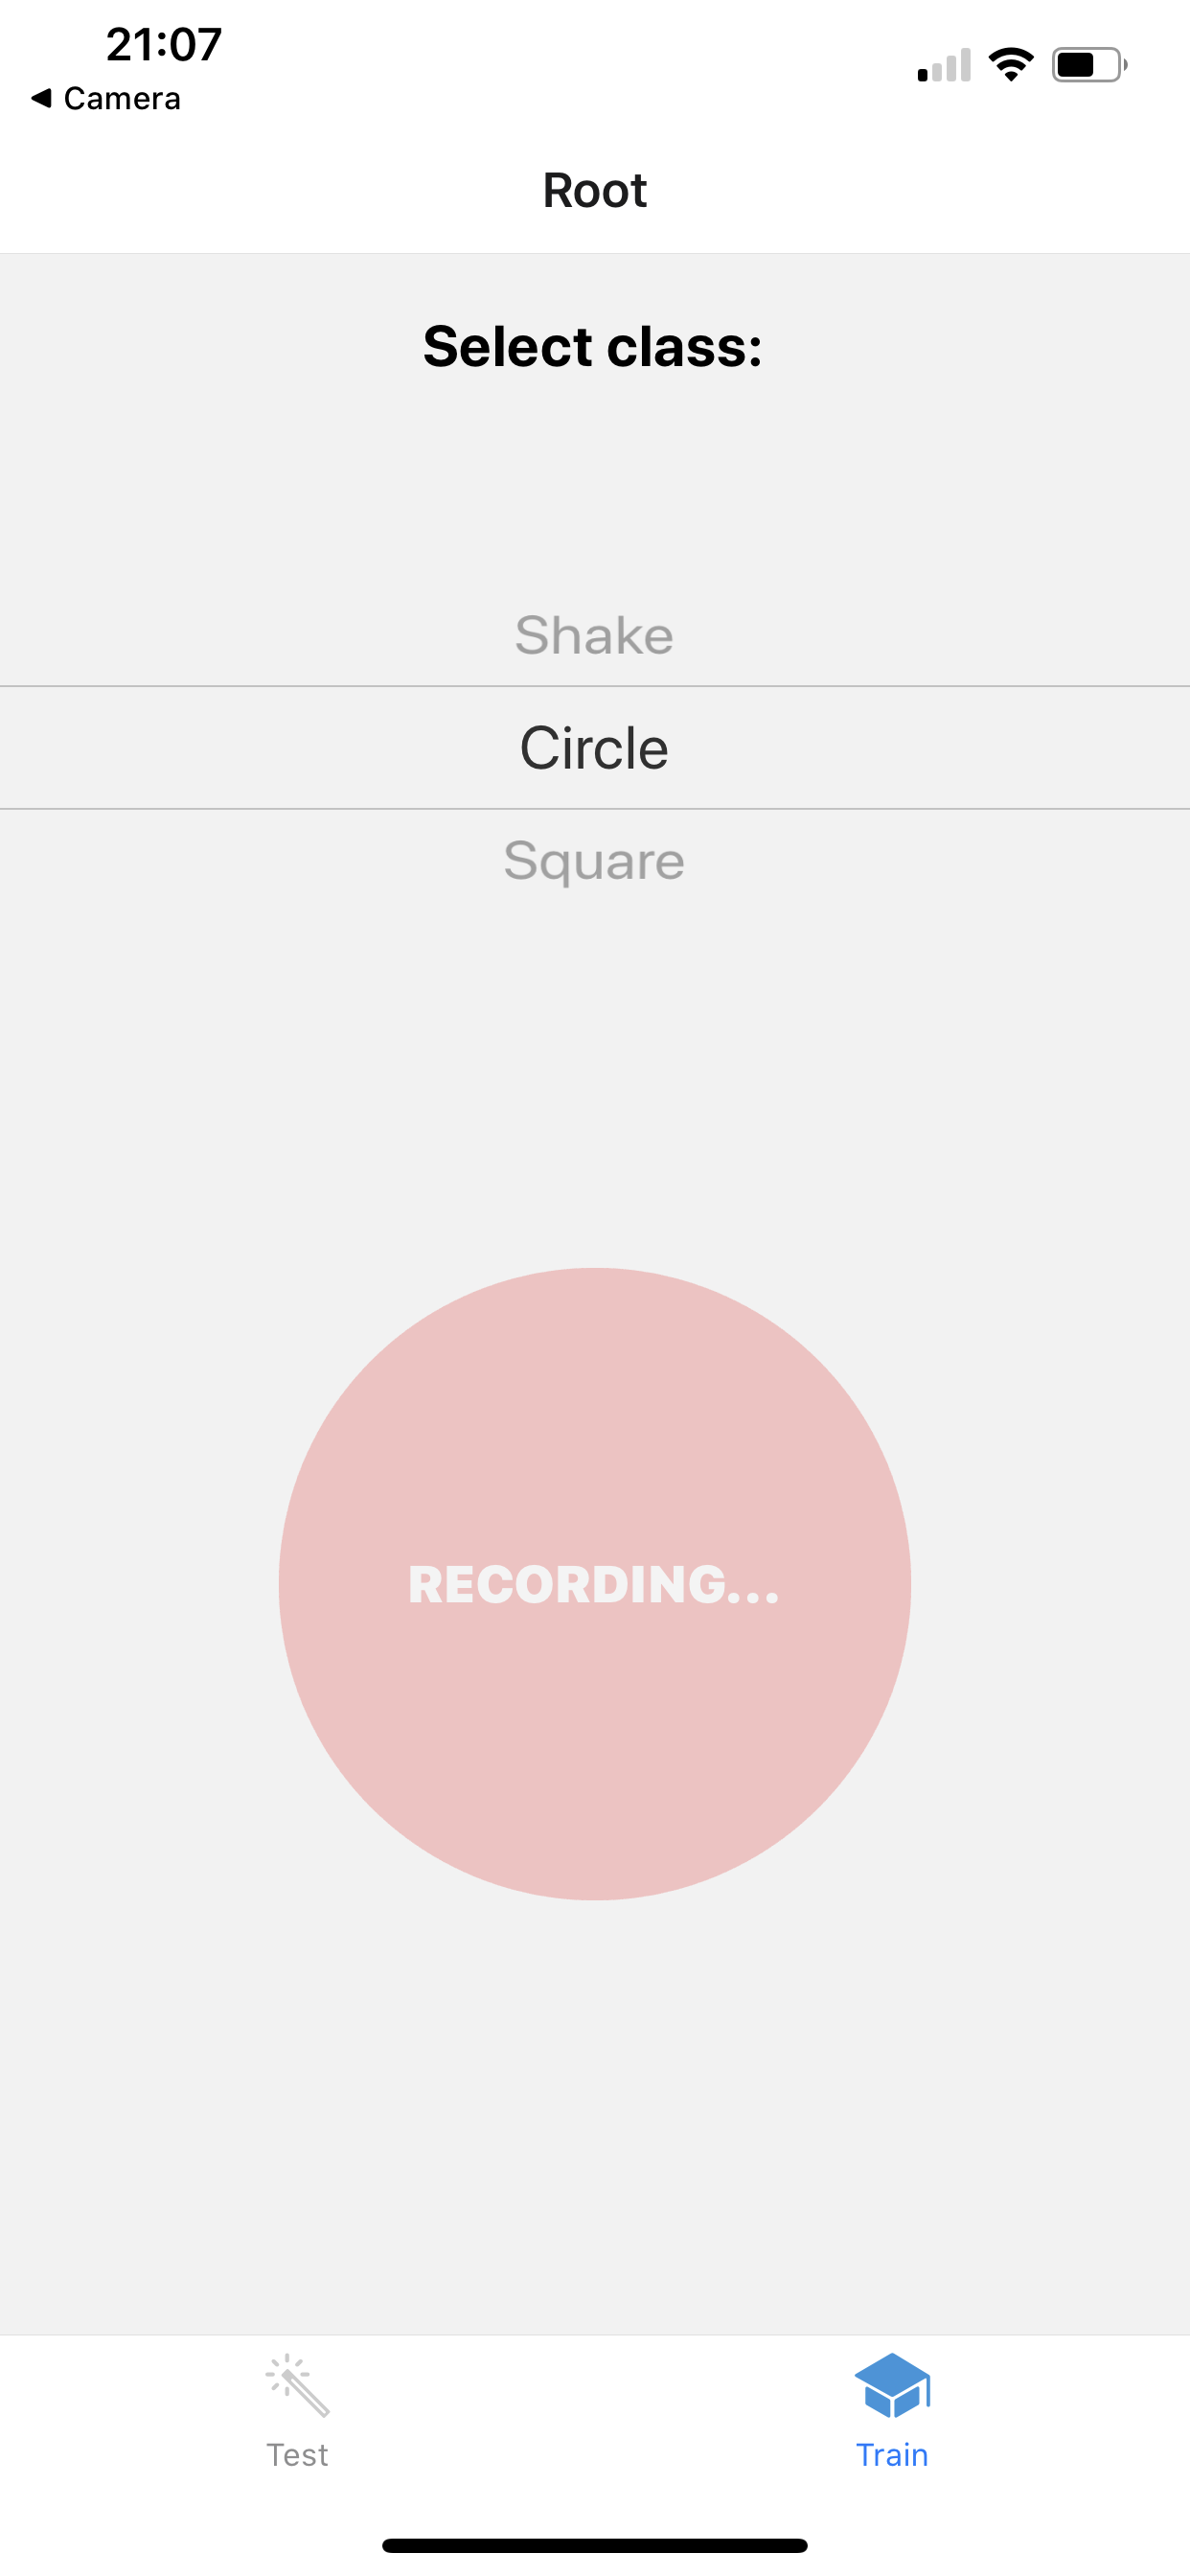
\includegraphics[width=0.15\textwidth]{testingapp_screenshots/IMG_2013.PNG} & 
            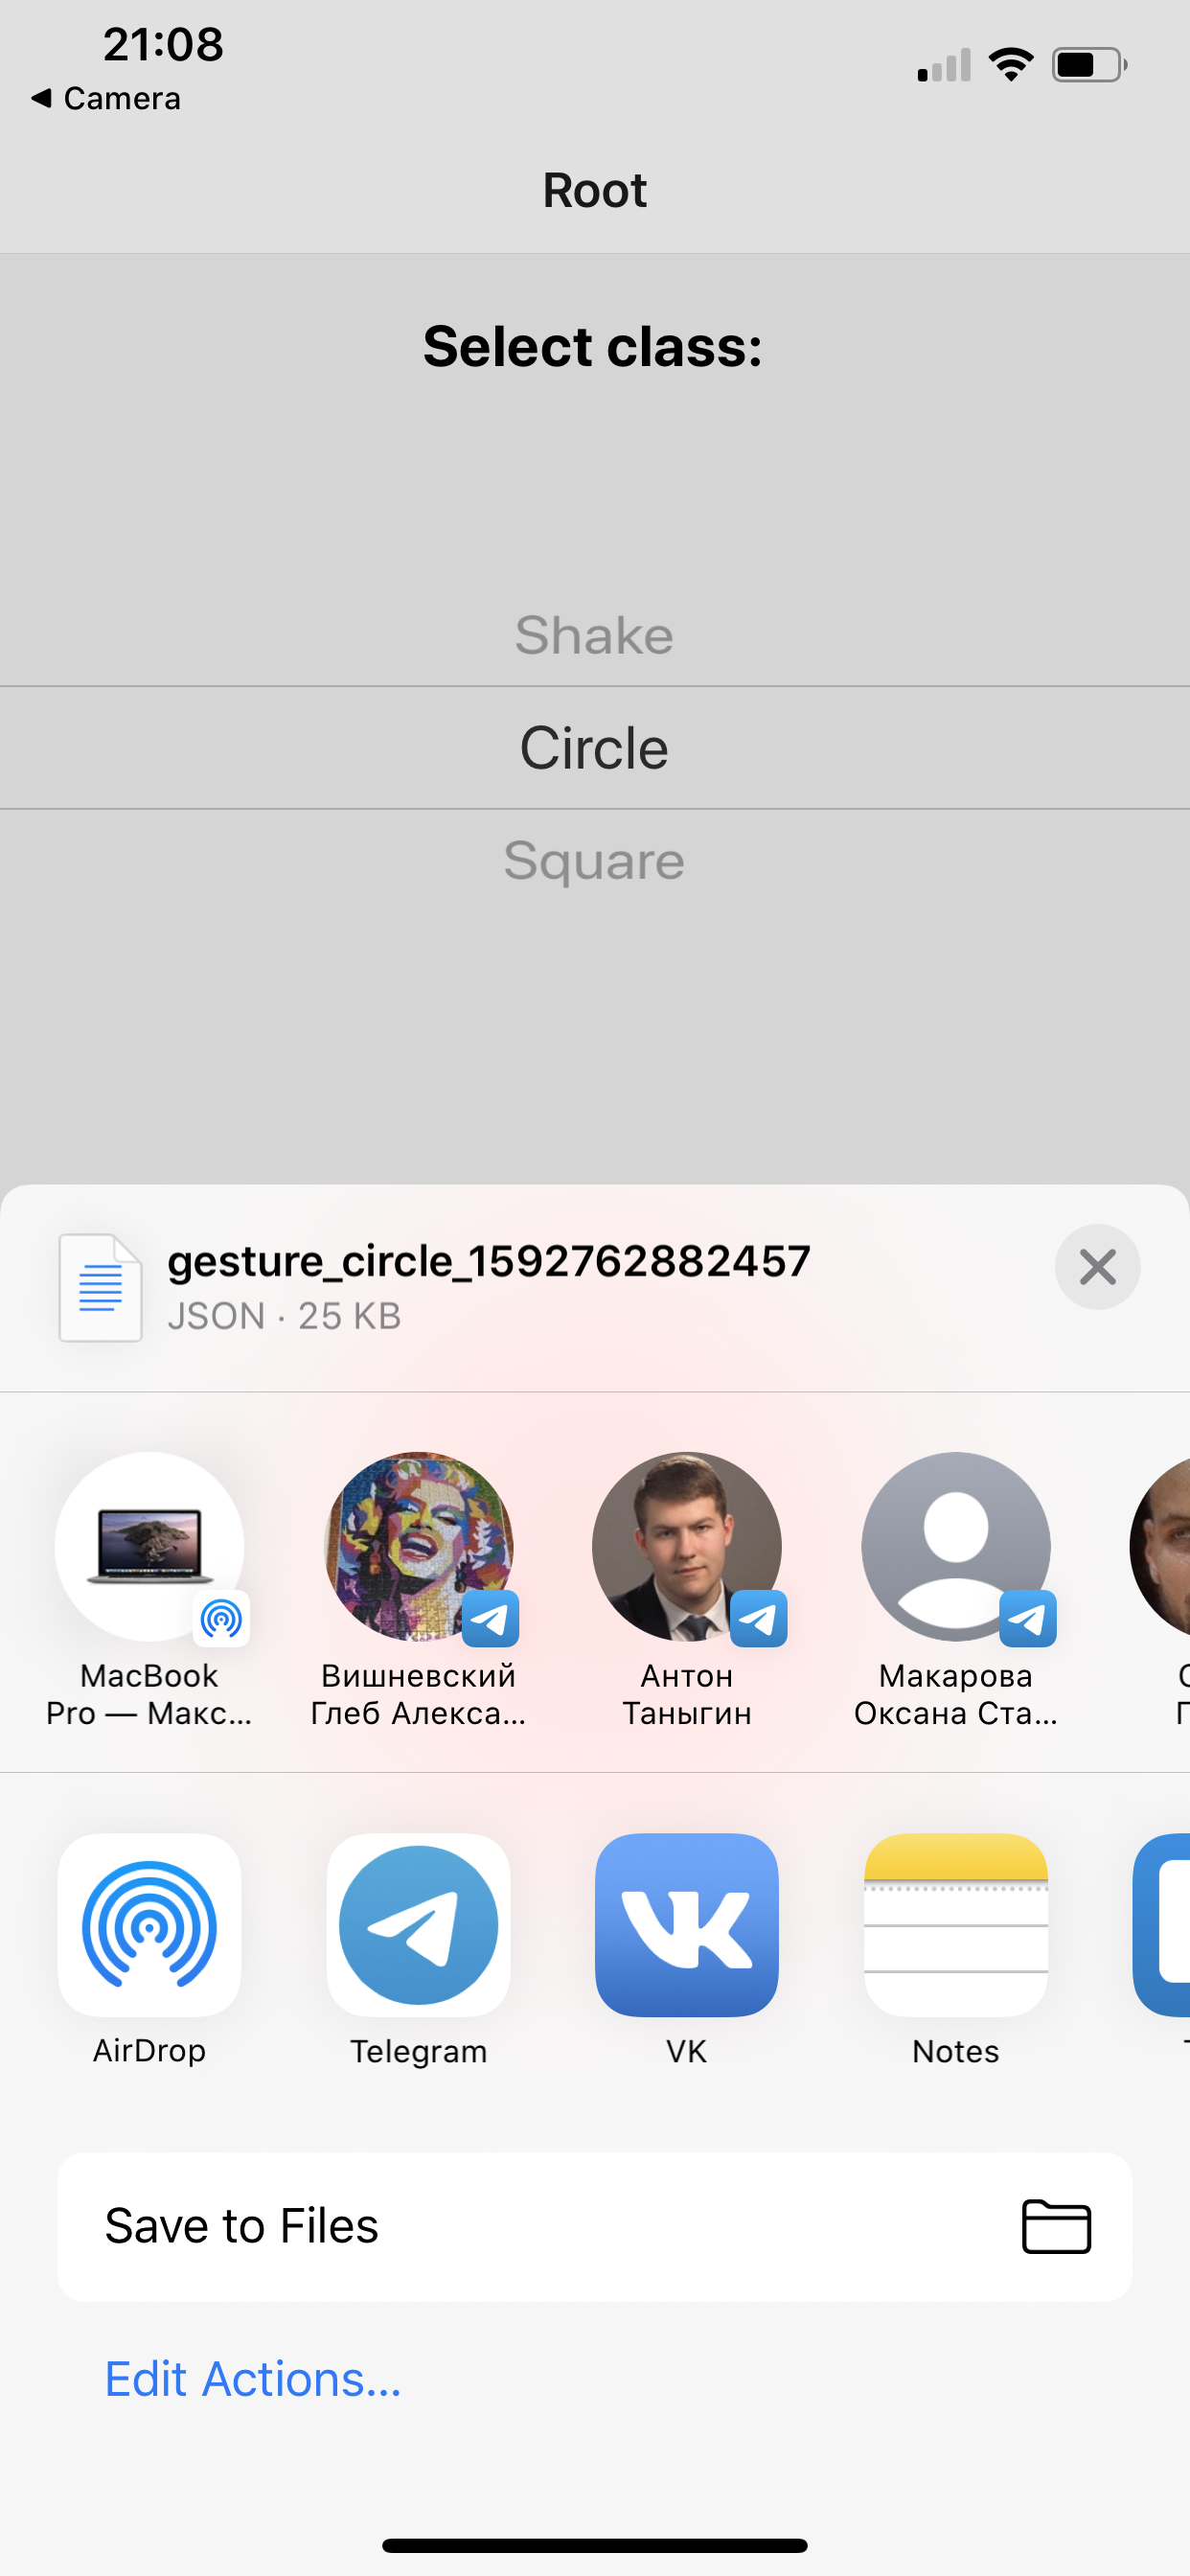
\includegraphics[width=0.15\textwidth]{testingapp_screenshots/IMG_2014.PNG} & 
            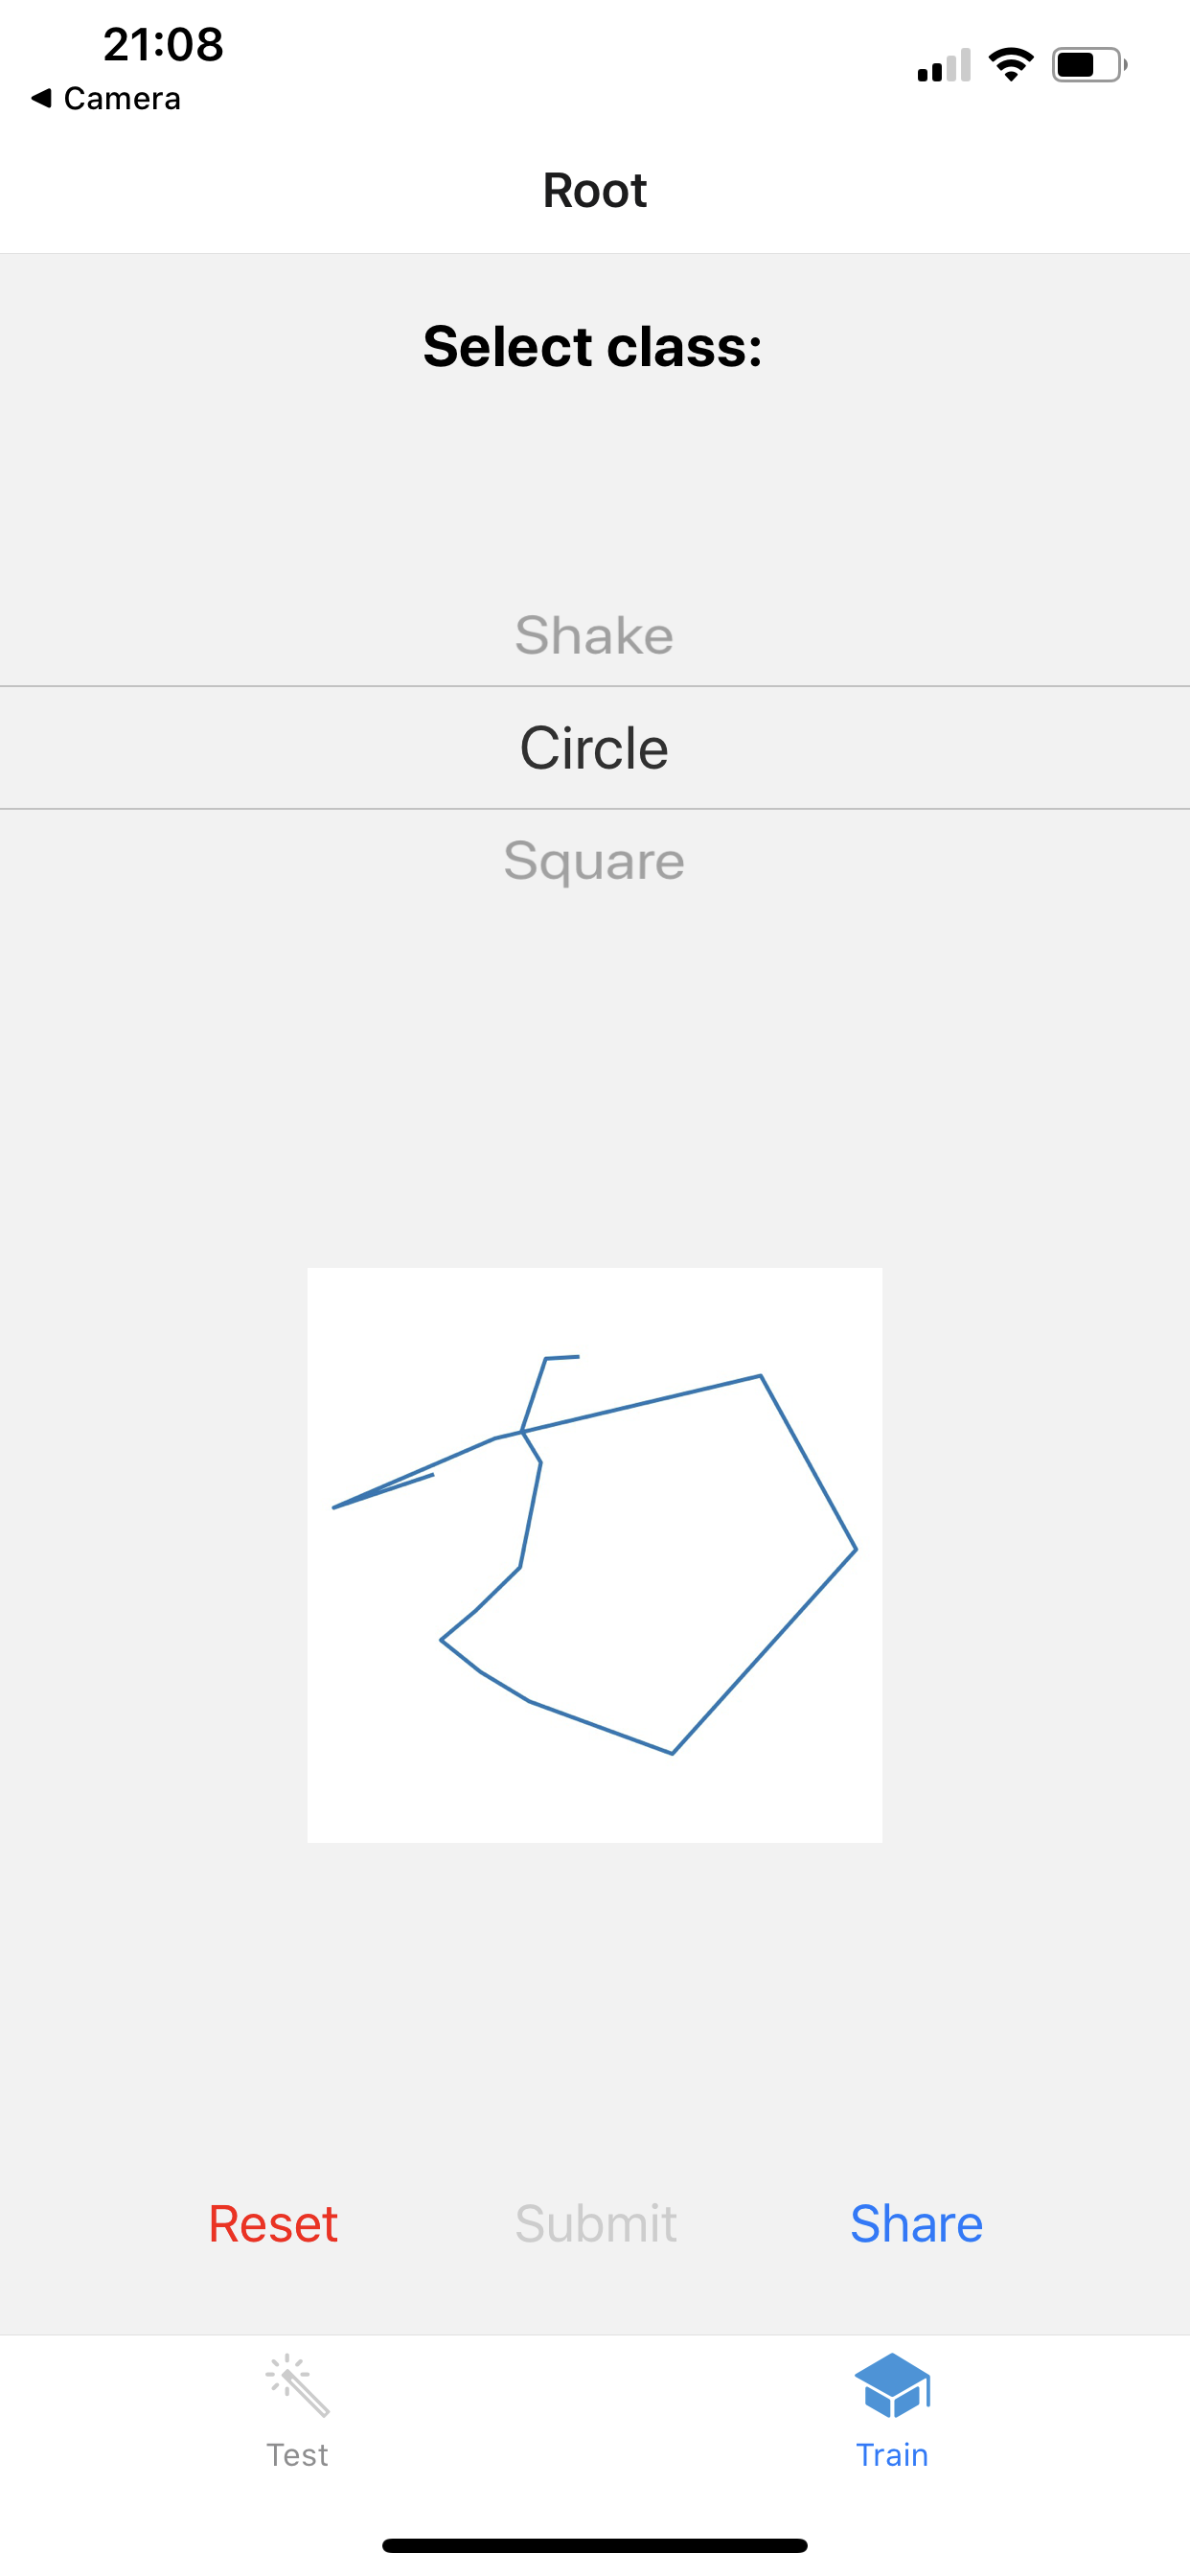
\includegraphics[width=0.15\textwidth]{testingapp_screenshots/IMG_2015.PNG} \\
        \end{tabular}
    \end{center}
    \caption{Интерфейс обучения в различных состояниях.}
\end{figure}